\documentclass[letterpaper,12pt,oneside]{article}

\usepackage[bookmarks=false]{hyperref}
\usepackage{styles/style}

\usepackage[
  top=2cm,
  bottom=2cm,
  left=2.5cm,
  right=2 cm,
  headheight=9pt, % as per the warning by fancyhdr
  includehead,includefoot,
  heightrounded, % to avoid spurious underfull messages
]{geometry} 

\newcommand{\institution}{Intituto Politécnico Nacional}
\newcommand{\schoolname}{Escuela Superior de Cómputo}
\newcommand{\shortschoolname}{ESCOM}
\newcommand{\shortinstitutionname}{IPN}
\newcommand{\program}{Ing. en Sistemas Computacionales}
\newcommand{\directors}
{
Rocío Palacios Solano\\
David Ortega Pacheco\\
}
% Datos de autores
\newcommand{\authors}
{
% INSTRUCTION: Colorar en orden alfabético
Gálvez Reyes Angel Alexander\\
Hernández Morales Osvaldo\\
}
% Datos de documento
\newcommand{\documenttitle}{Herramienta para la gestión de tratamientos e historial clínico dental}
\newcommand{\documentsubtitle}{Trabajo terminal}

\makeglossaries

\newglossaryentry{odontograma}
{
    name=Odontograma,
    description={Esquema utilizado por los odontólogos que permite registrar información sobre la boca de una persona}
}

\newglossaryentry{cariología}
{
    name=Cariología,
    description={Disciplina científica dentro de la odontología que trata acerca de las interrelaciones complejas entre los fluidos orales y los depósitos bacterianos y su relación con los cambios subsecuentes en los tejidos duros dentales que provocan la caries dental}
}

\newglossaryentry{anamnesis
Cómo se pronuncia
}
{
    name=Anamnesis,
    description={Conjunto de datos que se recogen en la historia clínica de un paciente con un objetivo diagnóstico.}
}


\newglossaryentry{periodontograma}
{
    name=Periodontograma,
    description={Tabla o gráfica que muestra el estado de tus encías y el nivel de tu hueso respecto al diente}
}

\newglossaryentry{periodonto}
{
    name=Periodonto,
    description={Conjunto de estructuras que van a servir de base al diente para que éste quede fijo a su alveolo, además cumple funciones demonológicas locales y es capaz de amortiguar la carga durante la masticación.}
}



\newglossaryentry{gloss01}
{
    name=Aplicación de página única,
    description={Aplicación que carga una única página HTML y todos los componentes necesarios (tales como JavaScript y CSS) para que se ejecute la aplicación. Cualquier interacción con la página o páginas subsecuentes no requiere hacer solicitudes al servidor lo que significa que la página no es recargada.}
}

\newglossaryentry{gloss02}
{
    name=ES6,
    description={Estas siglas se refieren a las más recientes versiones del estándar de Especificación de Lenguaje ECMAScript, del cual JavaScript es una implementación. La versión ES6 (también conocida como ES2015) incluye muchas adiciones a las versiones previas tales como: funciones flecha, clases, plantillas de cadena de texto, declaraciones de variables con let y const. }
}

\newglossaryentry{gloss03}
{
    name=Compiladores,
    description={Un compilador de JavaScript toma el código JavaScript, lo transforma y devuelve en un formato diferente. El caso de uso más común es tomar código JavaScript con sintaxis ES6 y transformarlo en código que navegadores más antiguos puedan interpretar. Babel es el compilador más usado con React. }
}

\newglossaryentry{gloss04}
{
    name=Bundlers,
    description={Los bundlers toman el código JavaScript y CSS escrito como módulos separados (frecuentemente cientos de ellos), y los combina en unos cuantos archivos mejor optimizados para los navegadores. Algunos bundlers comúnmente usandos en aplicaciones de React son Webpack y Browserify. }
}

\newglossaryentry{gloss05}
{
    name=Package managers,
    description={Los package managers son herramientas que te permiten administrar las dependencias de tu proyecto. npm y Yarn son dos package managers comúnmente usados en aplicaciones de React. Ambos son clientes para el mismo registro de paquetes npm. }
}
 
 \newglossaryentry{gloss06}
{
    name=CDN,
    description={CDN son las siglas en inglés de Content Delivery Network (Red de Entrega de Contenido). Los CDN entregan contenido estático en caché desde una red de servidores alrededor del mundo. }
}

\newglossaryentry{ coetaneidad}
{
    name= Coetaneidad,
    description={Que existe al mismo tiempo que otra cosa, o que pertenece a la misma época que ella.}
}



 \newglossaryentry{gloss07}
{
    name=JSX,
    description={JSX es una extensión de sintaxis para JavaScript. Es similar a un template language, pero tiene todo el poder de JavaScript. JSX es compilado a llamadas React.createElement() que regresan simples objetos de JavaScript llamados “elementos de React”.  }
}

 \newglossaryentry{gloss08}
{
    name=Componentes,
    description={Los componentes de React son pequeños y reutilizables fragmentos de código que devuelven un elemento de React para ser renderizado en una página.  }
}

 \newglossaryentry{gloss09}
{
    name=Props,
    description={Son entradas de un componente de React. Son información que es pasada desde un componente padre a un componente hijo. Los props son de sólo lectura. No deben ser modificados de ninguna forma. Para modificar algún valor en respuesta de una entrada del usuario o una respuesta de red, usa el estado en su lugar.
  }
}


 \newglossaryentry{gloss11}
{
    name=Elementos,
    description={Los elementos de React son los bloques de construcción de una aplicación de React. Uno podría confundir los elementos con el concepto más ampliamente conocido de “componentes”. Un elemento describe lo que quieres ver en pantalla. Los elementos de React son inmutables.  }
}

 \newglossaryentry{gloss10}
{
    name=Estado,
    description={Un componente necesita estado cuando algunos datos asociados a el cambian con el tiempo. Por ejemplo, un componente Checkbox tal vez necesite isChecked en su estado, y un componente NewsFeed tal vez necesite mantener un registro de fetchedPosts en su estado. La diferencia más importante entre estado y props es que los props son pasados desde un componente padre, pero el estado es manejado por el propio componente. Un componente no puede cambiar sus props, pero puede cambiar su estado.
  }
}


 \newglossaryentry{gloss12}
{
    name=Enterprise Resource Planning,
    description={Son los sistemas de información gerenciales que integran y manejan muchos de los negocios asociados con las operaciones de producción y de los aspectos de distribución de una compañía en la producción de bienes o servicios. Entre sus módulos más comunes se encuentran el de manufactura o producción, almacenamiento, logística e información tecnológica, incluyen además la contabilidad, y suelen incluir un sistema de administración de recursos humanos, y herramientas de mercadotecnia y administración estratégica.
  }
}

 \newglossaryentry{gloss13}
{
    name=Antecedentes heredo familiares,
    description={Registro de las relaciones entre los miembros de una familia junto con sus antecedentes médicos. Esto abarca las enfermedades actuales y pasadas. En los antecedentes familiares a veces se observa la distribución de ciertas enfermedades en una familia. También se llama historia médica familiar (Instituto Nacional del Cáncer de los Institutos Nacionales de la Salud de EE. UU.). 
  }
}


\newacronym{sires}{SIRES}{Sistemas de Información de Registro Electrónico para la Salud}

\newacronym{emr}{EMR}{Electronic Medical Records }

\newacronym{ehr}{EHR}{Electronic Health Records }

\newacronym{phr}{PHR}{Personal Health Records}

\newacronym{his}{HIS}{Hspital Information System}

\newacronym{cis}{CIS}{Clinical Information System}

\newacronym{xml}{XML}{Extensible Markup Language}

\newacronym{uml}{UML}{Unified Modeling Language}

\newacronym{hms}{HMS}{Hospital Management Software}

\newacronym{lis}{LIS}{Laboratory Information System}

\newacronym{ris}{RIS}{Radiology Information System}

\newacronym{pacs}{PACS}{Picture Archiving and Communication System}

\newacronym{erp}{ERP}{Enterprise Resource Planning}


\begin{document}

%
\includepdf[pages=-]{documents/portada-tt.pdf}
%\import{content/}{cover}
%\pagebreak


\begin{flushright}
  \emph{Dedicatoria ...}
  \thispagestyle{empty}
\end{flushright}
\newpage



%
\pagestyle{empty}


{\Huge Agradecimientos\par}
%\spacing{1.5}%\doublespacing

\vspace{2em}
{\large Directores\par}
\vspace{1em}

\begin{itemize}
\item Rocío Palacios Solano
\item José David Ortega Pacheco
\end{itemize}

\vspace{1em}
{\large Sinodales\par}
\vspace{1em}

\begin{itemize}
\item Ulises Vélez Saldaña
\item Yasmín Ivette Jiménez Galán
\item José Asunción Enríquez Zárate
\end{itemize}

\vspace{1em}
{\large Odontólogos\par}
\vspace{1em}

\begin{itemize}
\item Fabiola Miroslava Olivares García
\item Ricardo Esquivel Jaime
\item José Alonso Guillen Dolores
\end{itemize}

\vspace{1em}
{\large Reconocimiento especial a la\par}
\vspace{1em}
\begin{itemize}
\item Familia Reyes.
\item Familia Hernández.
\end{itemize}





\newpage


\pagebreak
\setcounter{page}{1}
\pagestyle{fancy}
%---------------------------------------------------------
% Es lo último en escribrise
\section{Introducción}

Como consecuencia del ambiente de competencia económico y del desarrollo tecnológico en México los sistemas de información están cada vez más integrados a la medida de las organizaciones modernas, ya no solo para modelar procesos manuales, sino que, también aprovechando la inmensa capacidad de análisis de información disponible, este proceso de inmersión tecnológica resalta la posibilidad de los sistemas de información para mejorar la rapidez, la calidad y los costos de bienes y servicios. Dentro del ámbito clínico odontológico los procesos que se llevan a cabo de manera periódica en un consultorio tienen como eje central los aspectos clínicos, pero también los aspectos administrativos, estos segundos aspectos representan en ocasiones un problema dentro de los consultorios dentales privados, para quienes deben de hacerse cargo de diferentes roles dentro de su mismo negocio, cuando esto sucede se identifica la gran diferencia entre atender en una clínica dental y dedicarse a administrarla.

\vspace{1em}

El uso de un sistema que permita la gestión de información administrativa, consulta y almacenamiento de historiales clínicos dentales permite al odontólogo disminuir el tiempo en procesos como la búsqueda de historiales específicos, al mismo tiempo que permite consolidar la información referente las consultas resguardándolas de manera unificada, disminuyendo la cantidad de consumibles (como papel, tóner o tinta) y reduciendo el espacio destinado para albergar la documentación física de la información, manteniendo su integridad, su disponibilidad y aumentando su confidencialidad (si es que se usan los mecanismos apropiados para cumplir con esta característica).

\vspace{1em}

Mediante la investigación y comparación de diferentes sistemas que ofrecen el apoyo a la gestión del consultorio médico dental, se concluyó que con respecto a la normativa, estos no promocionan, anuncian, ni mucho menos aseguran cumplir con los lineamientos de normas asociadas al sistema de información de registro electrónico de la salud, las cuales son normas de observancia obligatoria en todo el territorio nacional para todos los establecimientos que presten servicios de atención médica que formen parte del Sistema Nacional de Salud, así como para aquellas personas físicas o morales que dentro del territorio nacional cuentan indistintamente con los derechos de propiedad, uso, autoría, distribución y/o comercialización de dichos sistemas; estas normas tienen por objeto regular los sistemas de información de registro electrónico para la salud, así como establecer los mecanismos para que los prestadores de servicios de salud del sistema nacional de salud registren, intercambien y consoliden información.

\vspace{1em}

Los problemas que se pretenden atender con el trabajo propuesto son: la escasa disponibilidad de software de gestión de tratamientos e historial clínico dental a un costo accesible para odontólogos con bajo presupuesto, tales como recién egresados que quieran hacer uso de un software con las características mencionadas; falta de atención y oportunidad de mejora en detalles específicos correspondientes a la gestión de tratamientos e historial clínico como la capacidad de resguardar la información especificada en la norma oficial Mexicana NOM-024-SSA3-2012 en el apartado 6.5 Identificación de Pacientes y Profesionales de la Salud dental; atención a la posible mejora de usabilidad en la navegación de las herramientas de apoyo a la gestión de tratamientos e historial clínico dental usando como referencia las investigadas.

\vspace{1em}

Para la exploración de una solución a esta problemática se consultó a profesionales de área odontológica con el fin de recopilar opiniones prácticas sobre el desarrollo e implementación de un sistema informático que pueda cubrir los procesos más significativos del servicio brindado en consultorios dentales, es por ello que ante las condiciones descritas anteriormente surge la decisión de crear un sistema de información que apoye la gestión de las actividades que lleva acabo el administrador del consultorio dental, beneficiando principalmente al odontólogo administrador; ahorrando desde espacio físico para el almacenamiento del historial de los pacientes hasta tiempo considerable invertido en la búsqueda de la información requerida asociada a un paciente o a un tratamiento, relacionado con los procesos y normas médicas pertinentes.


\iffalse
En la medida que las tecnologías de software se actualizan, se encuentran cada vez más aplicaciones que integran los medios electrónicos para el apoyo en la gestión, administración y toma de decisiones en el sector salud.

\vspace{1em}

La Norma Oficial Mexicana NOM-024-SSA3-2012 establece los criterios científicos, tecnológicos y administrativos obligatorios en la elaboración, integración, uso y archivo del expediente clínico. Dicha norma es de observancia general en el territorio nacional y sus disposiciones son obligatorias para los prestadores de servicios de atención médica de los sectores público, social y privado, incluidos los consultorios, en los términos previstos en la misma. 

\vspace{1em}

El historial clínico es un documento médico legal, que surge del contacto entre el médico y el paciente. En ella se recoge la información necesaria para la correcta atención de los pacientes. El historial clínico es un documento válido, desde el punto de vista clínico y legal, que recoge información de tipo asistencial,
preventivo y social.

\vspace{1em}

En nuestro país los problemas de administración de información se encuentran principalmente en: el registro, disponibilidad, duración, legibilidad e integridad de la información dentro del expediente médico. Y el departamento de Servicio Médico de la Escuela Superior de Cómputo no es una excepción. 

\vspace{1em}

La aplicación de las tecnologías de la información en el sector de la salud, dan la pauta para una mejora en la calidad de la atención médica proporcionando sistemas informáticos que apoyan a las actividades de este
sector.

\vspace{1em}

El uso de las tecnologías aplicadas en sistemas de información dirigidos al ámbito de la salud proporciona al médico portabilidad de la información, que le sirve para tener un rápido acceso al historial médico de un paciente.
\fi

\subsection{Problemática}

Actualmente los procesos que realizan los médicos odontólogos recién egresados, o con recursos insuficientes para adquirir acceso a la mayor parte de sistemas de información especializados en su área invierten más tiempo en solucionar situaciones administrativas relacionadas con la gestión de información de sus pacientes en comparación con los odontólogos que cuentan con la asistencia de un sistema para este fin, ese tiempo bien pudiera ser usado para analizar y planificar acciones futuras en la gestión de su consultorio. 

\vspace{1em}

En México, los odontólogos que poseen un consultorio y que hacen uso de un sistema de información que resguarde un expediente clínico deberían acatar los parámetros establecidos en la normatividad mexicana sobre los sistemas de información de registro electrónico para la salud, la cual es de observancia obligatoria en todo el territorio nacional para todos los establecimientos que presten servicios de atención médica que formen parte del Sistema Nacional de Salud que adopten un Sistema de Información de Registro Electrónico para la Salud \cite{A02}. 

\vspace{1em}

Una gran cantidad de sistemas de información que albergan historiales clínicos del área dental, carecen de consideraciones explicitas a la normatividad mexicana, debido a que en algunos casos estos fueron desarrollados en otros países, sin embargo acatar los parámetros establecidos en dichas normas permiten ayudar a los consultorios a garantizar la interoperabilidad, procesamiento, interpretación, confidencialidad y seguridad mediante el uso de estándares y catálogos de la información de los registros electrónicos en salud.

\subsection{Solución propuesta}

Para solucionar el problema previamente explicado se propone el desarrollo de un sistema de información para historiales clínicos dentales que funcione como una herramienta que asista al odontólogo a resguardar, consultar y registrar los datos del estado actual de un paciente en sus tratamientos (odontograma), sus tratamientos en proceso, su evolución, y sus datos personales, así como también el manejo de las citas con los pacientes.

\vspace{1em}

Se trata de una herramienta que podrá funcionar como sistema independiente, o como un complemento de los sistemas que ya se tengan integrados en los consultorios dentales. En la herramienta se podrán gestionar los registros clínicos de los pacientes, lo que implica dar de alta registros de pacientes, eliminarlos, modificarlos y consultarlos. La información que se pueda guardar en la herramienta contemplará la normatividad mexicana correspondiente a los sistemas de información de registro electrónico para la salud sin pretender disponer de todos los elementos que cuenta un sistema certificado, el cuál además de contar con los catálogos correspondientes de datos, debe contar con el dictamen de verificación satisfactorio así como con la documentación de la información técnica requerida, de conformidad con lo dispuesto en la norma correspondiente y en las disposiciones jurídicas aplicables.

\begin{figure}[H]
\centering
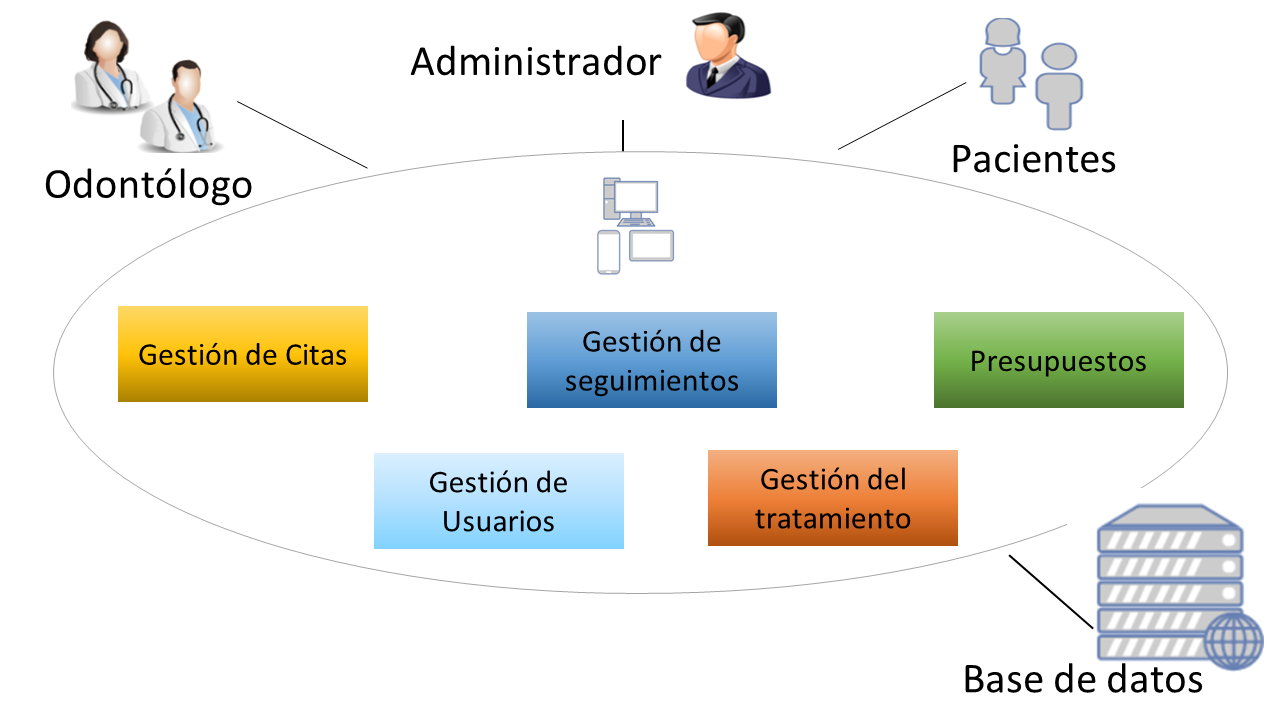
\includegraphics[width=12cm, keepaspectratio]{pictures/diagrama-protocolo.png}
\caption{Arquitectura básica de la herramienta}
\end{figure}

\subsection{Justificación}
%Mostrar los beneficios de realizar dicha aplicación
En México un aproximado de solo el 5\% de los egresados de odontología tienen la posibilidad de instalar su consultorio dental en un lapso de 5 años posteriores a la terminación de la carrera, por lo cual es necesario impulsar las condiciones necesarias para que este sector aumente su posibilidad de desarrollo, reducir los costos en administración y gestión del negocio, es una de las formas de apoyar la creación de condiciones de oportunidad \cite{D01}.  Por otra parte, el mayor porcentaje del mercado actual de clientes para clínicas de odontología tiene un perfil de edad entre 18-34, lo cual se traduce en un 73\%, clientes que ya hacen un uso frecuente de tecnologías digitales para interactuar con la mayoría de los negocios, principalmente tecnologías web \cite{D02}, este uso de la tecnología implica una oportunidad amplia de mejora en los procesos de servicios de salud, como es el caso del área odontológica.


\vspace{1em}

Los módulos considerados en el sistema propuesto pretenden ser útiles, y lo suficientemente flexibles para permitir que el sistema funcione ya sea como un sistema único para la gestión del consultorio, o también como una herramienta complementaria a los sistemas que pueda tenerse en el consultorio, que abarca la apertura de diagnósticos, registro de pacientes y usuarios, búsqueda de historiales clínicos, y gestión de citas. Los posibles beneficios de emplear más tiempo en la atención del paciente, permite potencialmente ofrecer un mejor servicio para los pacientes y proporcionar una alternativa de bajo costo, que haga consideración con los conceptos de la norma de salud establecida en relación con el registro electrónico de información


\subsection{Objetivo general}

Desarrollar una herramienta que permita apoyar las tareas de gestión de tratamientos e historial clínico dental para brindar una alternativa accesible a odontólogos con bajo presupuesto, que aporte a su vez, una propuesta de usabilidad sobre una interfaz que haga sencilla\footnote{''Para la elaboración este trabajo se realizó entrevistas a odontólogos en consultorios dentales, utilizaron la expresión de <<interfaz sencilla>> como sinónimo de menor cantidad de submenús anidados, y acceso casi inmediato al historial de un paciente.''} la operación de la herramienta.


\subsection{Objetivos particulares}

\begin{itemize}
\item Desarrollar un módulo de gestión de usuarios.
\item Desarrollar un módulo de gestión del tratamiento y citas
\item Desarrollar un módulo de gestión de presupuestos y seguimiento.
\end{itemize}


\newpage
\section{Marco teórico}
% El marco teórico, también llamado marco de referencia, es el soporte teórico, contextual o legal de los conceptos que se utilizaron para el planteamiento del problema en la investigación.

El marco teórico que fundamenta el sistema propuesto proporcionará los conceptos básicos, complementarios y específicos necesarios para el entendimiento del desarrollo de este trabajo. Se abordarán temas relacionados a los historiales clínicos, qué son, para qué sirven, y cómo se conforman, considerando el área dental, también se mencionará el uso de la información clínica en sistemas informáticos.

\subsection{Historial clínico}

El historial clínico, historia clínica o expediente clínico es un documento médico-legal donde queda registrada toda la relación del personal sanitario con el paciente, todos los actos y actividades médico-sanitarias realizados con él y todos los datos relativos a su salud \cite{D03}. El historial clínico dental funciona como una herramienta de uso cotidiano en las ciencias médicas donde se recopilan todos los datos de la historia de enfermedades, padecimientos, procedimientos llevados a cabo y tratamientos de un paciente.

\vspace{1em}

A continuación se mencionan algunas de las características que debe tener un historial médico tomando en cuenta consideraciones éticas en la práctica de las ciencias médicas:

\begin{itemize}
\item \textbf{Confidencialidad:} El secreto médico, la confidencialidad e intimidad y el historial clínico, son tres cuestiones que se implican recíprocamente y se relacionan.
            
\item \textbf{Disponibilidad:} Aunque debe preservarse la confidencialidad y la intimidad de los datos en ella reflejada, debe ser así mismo un documento disponible, facilitándose en los casos legalmente contemplados, su acceso y disponibilidad. 
            
\item \textbf{Único:} El historial clínico debe ser única para cada paciente por la importancia de cara a los beneficios que ocasiona al paciente la labor asistencial y la gestión.
             
\item \textbf{Legible:} Una historia clínica mal ordenada y difícilmente legible perjudica a todos, a los médicos, porque dificulta su labor asistencial y a los pacientes por los errores que pueden derivarse de una inadecuada interpretación de los datos contenidos en el historial clínico.
            
\item \textbf{Veracidad:} El historial clínico, debe caracterizarse por ser un documento veraz, constituyendo un derecho del usuario. El no cumplir tal requisito puede incurrir en un delito tipificado en el actual código Penal como un delito de falsedad documental.
            
\item \textbf{Coetaneidad de registros:} El historial clínico debe realizarse de forma simultánea y coetánea con la asistencia prestada al paciente.
            
\item \textbf{Completo:} Debe contener datos suficientes y sintéticos sobre la patología del paciente, debiéndose reflejar en ella todas las fases médico-legales que comprenden todo acto clínico-asistencial. Así mismo, debe contener todos los documentos integrantes del historial clínico, desde los datos administrativos, documento de consentimiento, informe de asistencia, protocolos especiales, etc.
             
\item \textbf{Identificación del profesional :} Todo facultativo o personal sanitario que intervenga en la asistencia del paciente, debe constar su identificación, con nombre y apellidos de forma legible, rúbrica y número de colegiado.
\end{itemize}

Dentro del marco de la normatividad mexicana, en específico, la norma NOM-004-SSA3-2012 del expediente clínico, define historial clínico como un conjunto único de información y datos personales de un paciente, que puede estar integrado por documentos escritos, gráficos, imagenológicos, electrónicos, magnéticos, electromagnéticos, ópticos, magneto-ópticos y de otras tecnologías, mediante los cuales se hace constar en diferentes momentos del proceso de la atención médica, las diversas intervenciones del personal del área de la salud, así como describir el estado de salud del paciente; además de incluir en su caso, datos acerca del bienestar físico, mental y social del mismo \cite{A04}.

\vspace{1em}

Para el caso de los denominados sistemas de información de registro electrónico para la salud SIRES, que son particularmente importantes para el presente trabajo, se tiene en consideración de referencia la norma NOM-024-SSA3-2012 de Sistemas de información de registro electrónico para la salud, Intercambio de información en salud. \cite{A05}.

\vspace{1em}

La norma mexicana NOM-024-SSA3-2012 establece los objetivos funcionales y funcionalidades que deberán observar los productos de historial clínico electrónico (HCE) o también conocidos como sistemas de expediente clínico electrónico para garantizar la interoperabilidad, procesamiento, interpretación, confidencialidad, seguridad y uso de estándares y catálogos de la información de los registros electrónicos en salud.

\vspace{1em}

La Norma Oficial Mexicana NOM-024-SSA3-2012 entró en vigor desde el 28 de enero de 2013 dejando sin efectos a la NOM-024-SSA3-2010. Dicta que los sistemas de expediente clínico electrónico deberán garantizar la confidencialidad de la identidad de los pacientes, así como la integridad y confiabilidad de la información clínica y, establecer las medidas de seguridad pertinentes y adecuadas a fin de evitar el uso ilícito o ilegítimo que pueda lesionar la esfera jurídica del titular de la información, de acuerdo con la normatividad aplicable.

\vspace{1em}

Por otra parte, la información contenida en los sistemas de expediente podrá ser dada a conocer al paciente, o a quien tenga facultad legal para decidir por él, y en su caso a terceros mediante orden de la autoridad judicial, o administrativa competente.

\vspace{1em}

El cumplimiento de esta norma es obligatoria para el sistema nacional de salud, prestadores de servicios de salud de carácter público, social y privado que adopten un sistema de registros electrónicos en salud.

\vspace{1em}

Los tipos de sistemas de expediente clínico electrónico que estarán sujetos a esta norma son aquellos destinados a los siguientes usos en el ámbito de la provisión de servicios de salud:

\begin{itemize}
\item Consulta Externa
\item Hospitalización
\item Urgencias
\item Farmacia
\item Laboratorio
\item Imagenología
\item Quirófano
\end{itemize}

En el caso de los consultorios dentales, estos se encuentran clasificados como servicios de salud de consulta externa.

La norma NOM-024-SSA3-2012, mencionada con anterioridad, hace referencia a otras normas, las cuales se en listan a continuación:

\begin{itemize}
    \item Norma Oficial Mexicana NOM-035-SSA3-2012, En Materia de Información en Salud: Establece los criterios y procedimientos que se deben seguir para producir, captar, integrar, procesar, sistematizar, evaluar y divulgar la Información en Salud, sin embargo su enfoque es dirigido a las condiciones y entorno físico del lugar donde se prestan servicios de atención a la salud en establecimientos fijos y/o móviles.
    \item Norma Oficial Mexicana NOM-004-SSA3-2012, Del Expediente Clínico: Esta norma, establece los criterios científicos, éticos, tecnológicos y administrativos obligatorios en la elaboración, integración, uso, manejo, archivo, conservación, propiedad, titularidad y confidencialidad del expediente clínico. Esta norma cuenta con más de 120 campos a considerar en el expediente clínico, y en e apartado integración para el historial clínico considera 11 campos, los cuales son:
    \begin{itemize}
        \item Ficha de Identificación
        \item Antecedentes heredo familiares
        \item Antecedentes personales no patológicos
        \item Antecedentes personales patológicos
\item Padecimiento actual.
\item Interrogatorio por aparatos y sistemas.
\item Exploración física (habitus exterior, signos vitales, datos de cabeza, cuello, tórax, abdomen, extremidades y genitales).
\item Resultados previos y actuales de estudios de laboratorio, gabinete y otros
\item Terapéutica empleada y resultados obtenidos (medicamento, vía, dosis, periodicidad).
\item Diagnóstico(s) o problemas clínicos.
\item Nombre completo, cédula profesional y firma del médico.
    \end{itemize}
    \item Norma Oficial Mexicana NOM-017-SSA2-1994, Para la Vigilancia Epidemiológica  (No tiene relación directa con el presente trabajo).
\end{itemize}




\subsection{Historial clínico dental}

El principal objetivo de la historia clínica odontológica es mejorar la atención sanitaria al paciente, ya que teniendo información sobre su estado actual y antecedentes es más fácil conseguir un diagnóstico y tratamiento adecuados. A efectos legales la historia médica también es de gran importancia dado que sirve como prueba de los procedimientos realizados sobre el paciente. Es por eso que cada nueva información añadida al historial debe ser firmada y fechada. Por otra parte, la historia clínica también se usa con fines de docencia e investigación, en cuyo caso hay que garantizar el anonimato del paciente.\cite{A06}

No hay una plantilla estándar para la realización de un historial clínico dental, pero se asume que para ser de utilidad tiene que cumplir con las características siguientes: 
\begin{itemize}
\item Debe ser único, integrado, acumulativo (se va completando a medida que se van realizando diagnósticos e intervenciones) y cronológica.
\item Debe contener información veraz.
\item Debe existir un sistema eficaz de recuperación de la información clínica.
\item Debe adjuntar los consentimientos informados obtenidos de acuerdo a la ley.
\item Debe estar siempre a disposición, para permitir una permanente evaluación y revisión crítica por parte de los profesionales.
\item Debe ser siempre escrito con letra clara y legible por parte de cualquier persona.
\item Cualquier historial clínico es por definición confidencial y tiene que almacenarse en un lugar seguro para evitar el acceso de terceras personas.
\end{itemize}

Como resultado de la investigación del trabajo se determina que los elementos básicos de un historial clínico dental son:

\begin{itemize}
\item Anamnesis: Recoge los datos más importantes del paciente (nombre, edad, datos de contacto, estado general de salud, hábitos…) junto con el motivo de asistencia a la consulta.
            
\item Exploración: Recoge todos los datos de interés que aparecen en la exploración del dentista. La exploración se divide en intraoral y extraoral.
            
      El estado de cada pieza dental se refleja en la odontograma, una representación esquemática de la dentadura del paciente en la que los dientes se identifican con dos cifras: la primera indica el cuadrante de la boca en el que se encuentra el diente y la segunda el tipo de diente (muela, incisivo…). El odontograma es la herramienta principal de la cariología, la cuál es la disciplina científica dentro de la odontología que trata acerca de las interrelaciones complejas entre los fluido sorales y los depósitos bacterianos y su relación con los cambios subsecuentes en los tejidos duros dentales que provocan la caries dental.
            
      \begin{figure}[H]
      \centering
      \centerline{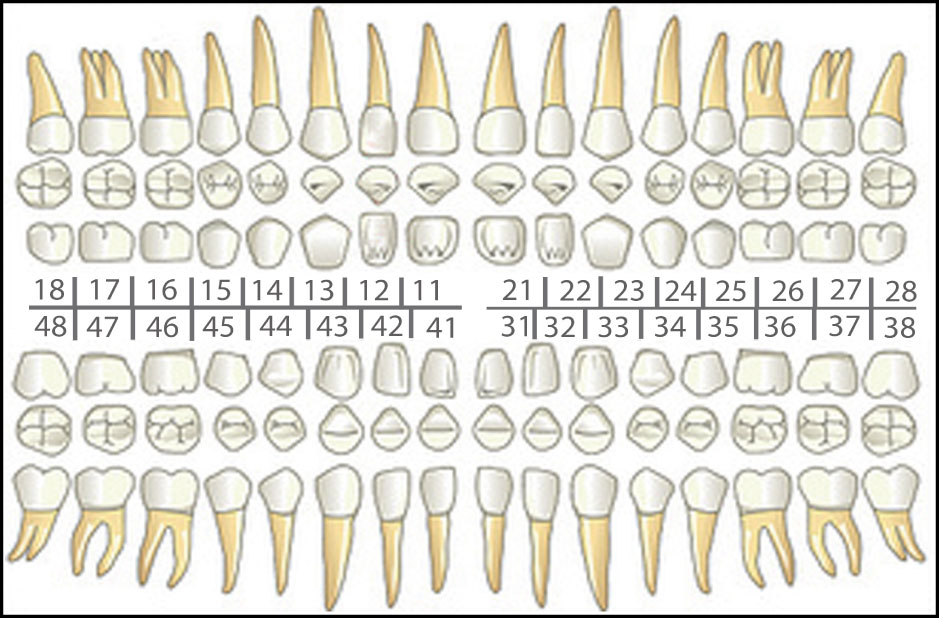
\includegraphics[width=12cm, keepaspectratio]{pictures/picture15.jpg}}
      \caption{Ejemplo de odontograma}
      \end{figure}
            
      El estado de salud de las encías y también cavidad bucodental, se muestra en el periodontograma, se trata de una tabla o gráfica que muestra el estado de tus encías y el nivel de tu hueso respecto al diente. También analiza la presencia de sangrado y otros parámetros. El periodontograma es la herramienta principal de la periodontología, la cuál es la especialidad contemporánea de la odontología que emerge de la periodoncia para sustentar el estudio de evidencia científica sobre el estado del periodonto sano y enfermo. La periodoncia es la especialidad clínica para diagnosticar, prevenir y tratar las enfermedades y condiciones que afectan al periodonto.
            
      \begin{figure}[H]
      \centering
      \centerline{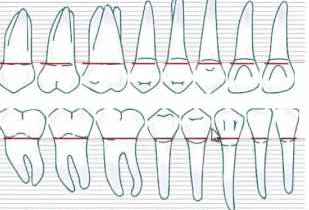
\includegraphics[width=9cm, keepaspectratio]{pictures/picture16.png}}
      \caption{Ejemplo de periodontograma}
      \end{figure}
            
\item Diagnóstico: Con la información de los dos apartados anteriores el dentista puede emitir un diagnostico que queda debidamente reflejado en el historial clínico.
            
\item Plan de tratamiento: Tras el diagnostico llega el momento del tratamiento prescrito (si es que se necesita alguno), que también se anota en la historia.
\end{itemize}

En cuanto al formato, aunque aún es posible ver historias clínicas dentales en papel e incluso escritas a mano, en la actualidad se prefiere usar el soporte informático. Lo que se conoce como historia clínica digital, electrónica o informatizada.



\subsection{Sistemas de información}

Como se mencionó anteriormente, los sistemas informáticos son conjuntos de software (es el componente lógico, el sistema operativo, el firmware y las aplicaciones) hardware (o componente físico, como dispositivos electrónicos como la memoria, los sistemas de almacenamiento externo, los procesadores) y la persona o recurso humano que los ejecuta, y que interrelacionadas funcionan entre sí con un objetivo determinado, permitiendo el proceso y el almacenamiento de información.

\vspace{1em}

La transición a los registros médicos electrónicos ha introducido a los profesionales y sus clientes a varios acrónimos que ahora están firmemente arraigados en el léxico de la atención médica.

Un registro médico electrónico (EMR por sus síglas en inglés electronic medical record) es la forma digital de los registros clínicos en papel que las instalaciones de atención médica usaban anteriormente para realizar un seguimiento de los tratamientos, medicamentos, cambios en la condición, etc. Un registro médico electrónico representa una actualización sobre el documento en papel tradicional porque lo hace fácil para los profesionales rastrear los datos a lo largo del tiempo y monitorear la salud del cliente de manera más confiable, lo que conduce a una mejor atención a largo plazo.

\vspace{1em}

Al igual que un EMR, un registro de salud electrónico (EHR por sus síglas en inglés electronic health record) proporciona un registro digital de información de salud. Sin embargo, el EHR incluye más datos que el EMR ya que contiene información de todos los profesionales que participan en la atención del cliente. Por lo tanto, el EHR ofrece una visión más completa del historial de salud y tratamiento del cliente. Esta información se ingresa en una base de datos común que se puede compartir entre usuarios autorizados en varias organizaciones de atención médica.\cite{D04}

\vspace{1em}

Si bien un registro de salud personal (PHR por sus síglas en inglés personal health record) también proporciona un registro electrónico de la información relacionada con la salud del cliente, la diferencia es que, a diferencia de los EMR y EHR que son administrados y mantenidos por los profesionales, el cliente administra el PHR. El PHR permite a cada cliente ver y controlar los datos en un entorno seguro y compartirlos con otras partes cuando sea necesario. Un PHR puede contener información de múltiples fuentes, como médicos, dispositivos de monitoreo en el hogar y otros datos proporcionados por el cliente.

\vspace{1em}

Otra clasificación del software en el sector de la salud son los sistemas de información hospitalarios (HIS por sus síglas en inglés hospital information system o HMS por sus síglas en inglés hospital management software) y los sistemas de información clínicos (CIS por sus síglas en inglés Clinical Information System). 

\vspace{1em}

Un sistema de información clínica es un sistema basado en computadora que está diseñado para recopilar, almacenar, manipular y poner a disposición información clínica importante para el proceso de prestación de atención médica.

\vspace{1em}

En general los CIS proporcionan un depósito de datos clínicos que almacena datos clínicos como el historial de enfermedad del paciente y las interacciones con los proveedores de atención. El repositorio codifica información capaz de ayudar a los médicos a decidir sobre la condición del paciente, las opciones de tratamiento y las actividades de bienestar, así como el estado de las decisiones, acciones emprendidas y otra información relevante que podría ayudar a realizar esas acciones.

\vspace{1em}

Los CIS pueden estar limitados en un área única (por ejemplo, sistemas de laboratorio, sistemas de gestión de ECG) o pueden estar más extendidos e incluir prácticamente todos los aspectos de la información clínica de un EHR.

\vspace{1em}

El HIS es un sistema de información integral e integrado diseñado para administrar todos los aspectos de la operación de un hospital, tales como problemas médicos, administrativos, financieros y legales y el procesamiento correspondiente de los servicios. 

\vspace{1em}

Los HIS a menudo se componen de uno o varios componentes de software con extensiones específicas de especialidad, así como de una gran variedad de subsistemas en especialidades médicas de un mercado de múltiples proveedores. Nombre de implementaciones especializadas, por ejemplo , sistema de información de laboratorio, sistema de gestión de políticas y procedimientos, sistema de información de radiología o sistema de archivo y comunicación de imágenes. En términos en sistemas más generales y básicos podríamos decir que el HIS es un ERP especializado en el área médica.

\vspace{1em}

Considerando las diferencias en las características de los diferentes sistemas de información del área médico, podemos catalogar la herramienta dental como un EMR.

\vspace{1em}

El uso de un EMR compartido por múltiples instituciones y la interoperabilidad de los documentos electrónicos que componen el EMR, independientemente de las plataformas de software que utilicen, hace necesario que los sistemas de información que utilizan las instituciones de prestación de servicios de salud, en específico en el área dental, los consultorios deben implementar estándares informáticos, con el fin de garantizar la integridad y legibilidad de la información.

\vspace{1em}

A nivel internacional existen estándares como HL7 (Health Level Seven), el cuál representa un conjunto de estándares para facilitar el intercambio electrónico de información clínica, que utiliza una notación formal del lenguaje unificado de modelado (Unified Modeling Language, UML) y un metalenguaje extensible de marcado con etiquetas (Extensible Markup Language, XML), sin embargo para fines del trabajo presente solo se tomará en consideraciones catálogos de la norma mexicana NOM-024-SSA3-2012 de Sistemas de información de registro electrónico para la salud, Intercambio de información en salud.


\begin{figure}[H]
\centering
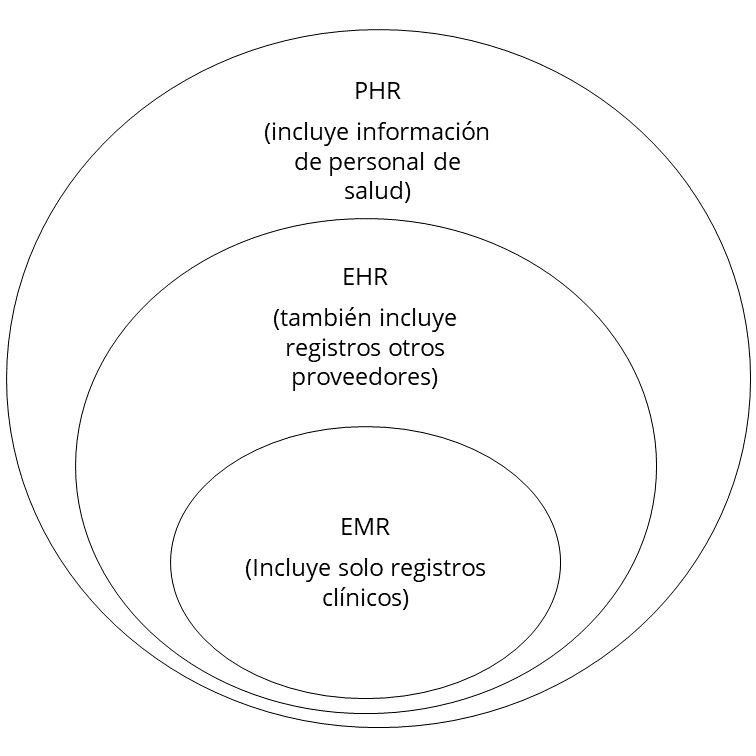
\includegraphics[width=10cm, keepaspectratio]{pictures/picture01.png}
\caption{Porcentajes de sitios web que utilizan varios servidores web desglosados por clasificación}
\end{figure}




\newpage
\section{Estado del arte}
% Es la recopilación de resultados de investigaciones hechas para comprender, interpretar, explicar o dar solución a un problema de investigación.

Se han realizado numerosos artículos de investigación, tesis académicas y trabajos terminales para titulación dentro del instituto, que tratan el tema de la incorporación de herramientas de software a la gestión de información de historiales médicos, sin embargo es tarea derivada del propósito de este trabajo, dar cuenta de la necesidad continua del surgimiento de nuevas herramientas que atiendan de manera particular el ámbito de la gestión de historiales clínicos dentales en México dentro del marco normativo concerniente al uso de sistemas de información de registro electrónico para la salud. 

\subsection{Artículos relacionados}

\noindent 
Algunos artículos publicados en repositorios bibliográficos institucionales y de asociaciones reconocidas en el ámbito tecnológico, científico, institucional y del sector con fecha de publicación menor a 5 años son:


\begin{longtable}{|p{4cm}|p{4cm}|p{8cm}|}
\hline\textbf{Título del artículo} & \textbf{Autores} & \textbf{Resumen} \\ \hline
Clinical Documentation of Dental Care in an era of EHR Use 
& Oluwabunmi Tokede\newline Rachel B. Ramoni\newline Michael Patton\newline John D. Da Silva\newline Elsbeth Kalenderian 
& Mediante una encuesta validada y un proceso Delphi de dos rondas, se exploran las características que debe contener un registro clínico dental en un registro electrónico de salud y la frecuencia de actualización de cada entrada como respuesta a la falta de estándares de documentación universalmente aceptados en este tipo de sistemas.\\ \hline
Integrating Dental Working Experience in Development of A Dental Clinic
Database System for A General Tertiary Hospital 
& Deena M. Barakah
& Resultado de una investigación en algunos departamentos de un grupo de hospitales y clínicas en Riad (la ciudad capital de Arabia Saudita), se propone la implementación de un sistema gestor de base de datos aplicado a una clínica dental.\\ \hline
Benefits of using an electronic health record 
& Robin Hoover
& En este artículo se resaltan algunos beneficios de usar sistemas de registros electrónicos de salud que se dirigen a los médicos, a los pacientes y a el manejo general de datos de índole médica.\\ \hline
\caption{Resumen de artículos relacionados.}
\label{table:1}
\end{longtable}


\subsection{Tésis relacionadas}

En la siguiente tabla se muestran algunas tesis que se han desarrollado con temas relacionados en los últimos 5 años:

\begin{longtable}{|p{4cm}|p{6cm}|p{6cm}|}
\hline\textbf{Título de la tesis} & \textbf{Autores} & \textbf{Resumen} \\ \hline
Propuesta de un CRM en una clínica dental 
& Edgar Manuel Cortéz Elizarraraz\newline Mónica Maribel Pérez Cruz\newline Alan Joel Valdivia Pérez \newline Javier Nain García Anaya
& Propuesta de implementación de un modelo para la clínica Dental Protec con la intención de mejorar el seguimiento de clientes, brindar un servicio adicional, y mejorar las campañas de marketing entre otras opciones.\\ \hline
Implementar un sistema web para la gestión clínica dental, aplicando tecnologías open source: caso “Consultorio Odontológico Navarro”
& Eduardo Javier Gonzales T. 
& Se contempla la construcción de un software para controlar el ingreso de datos personales de usuarios, creación de consultas, separación de citas médicas y atención en especialidades con su respectivo historial clínico.\\ \hline
Propuesta de un diseño de expediente clínico móvil para la prevención de enfermedades de los derechohabientes
& David Alexis Flores Martinez\newline Jose Carlos García Paz\newline Adriana Jazmin Neri Silva\newline Victor Josué Perez Sanchez\newline Eder Quintana Nequiz
& Propone una versión de expediente clínico electrónico, considerando nomenclatura médica, y partes de estándares de transmisión de datos médicos, clínicos y de imágenes.\\ \hline
\caption{Resumen de tesis relacionadas.}
\label{table:1}
\end{longtable}

\subsection{Trabajos terminales relacionados}

A continuación se muestra una tabla con algunos trabajos terminales de la Escuela Superior de Cómputo relacionados con el tema, en este caso en rango fechas de publicación y disponibilidad no han sido tan recientes:

\newpage
%\setlength\LTleft{-1cm}
%\setlength\LTright{0pt plus 1fill minus 1fill}
\setlength\LTleft{-0.5cm}
\begin{longtable}{|p{4cm}|p{5cm}|p{7.5cm}|}
\hline\textbf{Título del trabajo terminal} & \textbf{Autores} & \textbf{Resumen} \\ \hline
Sistema de gestión de servicios médicos para clínicas del CICS, Unidad Santo Tomás
& Cruz Pérez Jesús\newline M. V. Héctor Alejandro\newline Rosales A. Sergio Octavio
& Propuesta de software para el proceso de citas de las clínicas del CICS unidad Santo Tomás, considerando el manejo de materiales farmacológicos con el apoyo de gráficas para visualizar indicadores de las operaciones.\\ \hline
Aplicación móvil para la administración del historial clínico dental con animaciones demostrativas de tratamientos dentales (AMAAD)
& Enrique Martínez Gutiérrez\newline Soriano Arizabalo Nadehisa
& Propuesta de aplicación para IPad, para recaudar información de pacientes por medio de animaciones tridimensionales para facilitar a los pacientes la compresión de su tratamiento.\\ \hline
Sistema de expedientes clínicos electrónicos para el servicio de oftalmología
& Cazares Gomez Alfredo\newline Herrera Flores Patricia
& Propuesta de sistema de información para la gestión del servicio de oftalmología considerando la norma oficial mexicana NOM-024-SSA3-2012 del expediente clínico y la norma NOM-024-SSA3-2010 del expediente clínico electrónico.\\ \hline
Historial clínico para el departamento de servicio médico en ESCOM
& Jarquín García Osman
& Aplicación con tecnología móvil considerando la norma mexicana NOM-024-SSA3-2012, para resguardar información de historiales clínicos en el departamente de servicio médico de la ESCOM.\\ \hline
Sistema móvil de registros en enfermería implementando tecnología RFID
& C. G. Juan Carlos\newline Crespo Hernández Raquel\newline Rojas Alejo Diana Isabel
& Sistema híbrido (hardware y software) para consultar registros de enfermería mediante una aplicación móvil en Android empleando un tag de tecnología RFID.\\\hline
Sistema de expediente clínico con adquisición automática de datos
& M. C. Ariadna Betzabe\newline T. M. E. Eduardo Javier
& Análisis y diseño de un sistema de expediente clínico considerando la norma oficial mexicana NOM-024-SSA3-2012 del expediente clínico, por medio de una aplicación móvil para la medicion de algunos parámetros que se registran en los expedientes.\\\hline
\caption{Resumen de trabajos terminales relacionados.}
\label{table:1}
\end{longtable}

\newpage
\subsection{Software relacionado}

Ejemplos de software de registros clínicos que funcionan como soluciones enfocadas a el área de odontología, con disponibilidad y soporte en México y América latina:

\setlength\LTleft{0cm}
\begin{longtable}[H]{|p{0.30\textwidth}|C{0.20\textwidth}|C{0.20\textwidth}|C{0.20\textwidth}|}
\hline & Dentatec         & Dentalink         & Dentidesk         \\ 
\hline
Alojamiento de los datos           & Es responsabilidad del usuario & Es responsabilidad del proveedor del software & Es responsabilidad del proveedor del software 
\\ \hline 
Odontograma          & Si & Si  & Si  
\\ \hline
Presupuestos         & Si & Si  & Si  
\\ \hline
Agenda & Si & Si  & Si  
\\ \hline
Reportes descargables& Si & Si  & Si  
\\ \hline
Gestión de sucursales             & No & Si  & Si  
\\ \hline
Búsqueda de pacientes registrados & Si & Si  & Si  
\\ \hline
Historiales de pacientes con fotos & Si & Si  & Si  
\\ \hline
Enfoque clínico     & Si & Si  & Si  
\\ \hline
Enfoque administrativo             & Si & Si  & Si  
\\ \hline
Enfoque Educativo    & Si & No  & No  
\\ \hline
Respuesta automáticas             & No & No  & Si  
\\ \hline
\caption{Características de sistemas relacionados con la gestión de consultorios dentales.} \label{table:1} 
\end{longtable}


\newpage
\section{Análisis}

\subsection{Modelos de proceso de negocio}

El modelo y notación de procesos de negocio (BPMN por sus siglas en inglés Business Process Model and Notation), es una notación gráfica estandarizada que permite el modelado de procesos de negocio, en un formato de flujo de trabajo. Esta notación ha sido especialmente diseñada para coordinar la secuencia de los procesos y los mensajes que fluyen entre los participantes de las diferentes actividades.

\vspace{1em}

La diferencia principal entre el modelado de sistemas en UML y modelado de procesos de negocio con BPMN es que se hace más énfasis en como se realiza el trabajo en una organización, en lugar de que trabajo se hace. BPMN está dirigido a los analistas de negocio, arquitectos de sistemas e ingenieros de software. Fue desarrollado para mejorar el ciclo de vida del desarrollo de procesos desde el diseño de los mismos. BPMN está emparentado con UML por el hecho que ambos definen una notación gráfica para los procesos de negocio, sin embargo, BPMN y UML usan enfoques diferentes para modelarlos. UML en general ofrece un enfoque orientado a objetos para modelar aplicaciones, mientras que BPMN toma un enfoque centrado en los procesos.

\subsubsection{Modelo actual}

En los siguientes diagramas se describen los procesos tradicionales y genéricos que se siguen al realizar un tratamiento en un consultorio dental.

\vspace{1em}

Documentar ésta información es importante para identificar las partes del proceso de gestión de historiales clínicos dentales, y así seleccionar las partes en las que se debe enfocarse al realizar el análisis y diseño del trabajo.

\vspace{1em}

\noindent\textbf{Proceso general actual de tratamiento odontológico:} El proceso general actual de tratamiento odontológico, considera el primer contacto con el paciente ya que desde momento ese se maneja información, al establecer una primera cita, conoce el nombre de quien recibirá dicha cita, se programa en una agenda, ya sea una libreta, un calendario en físico y otras alternativas, para posteriormente, registrar el resto de los datos personales, llevar a acabo un diagnóstico, y un tratamiento que finaliza hasta que el paciente, ha recibido con éxito un procedimiento dental acordado, ha llegado a un estado de salud sano, o ha decidido terminar el tratamiento.

\begin{figure}[H]
\centerline{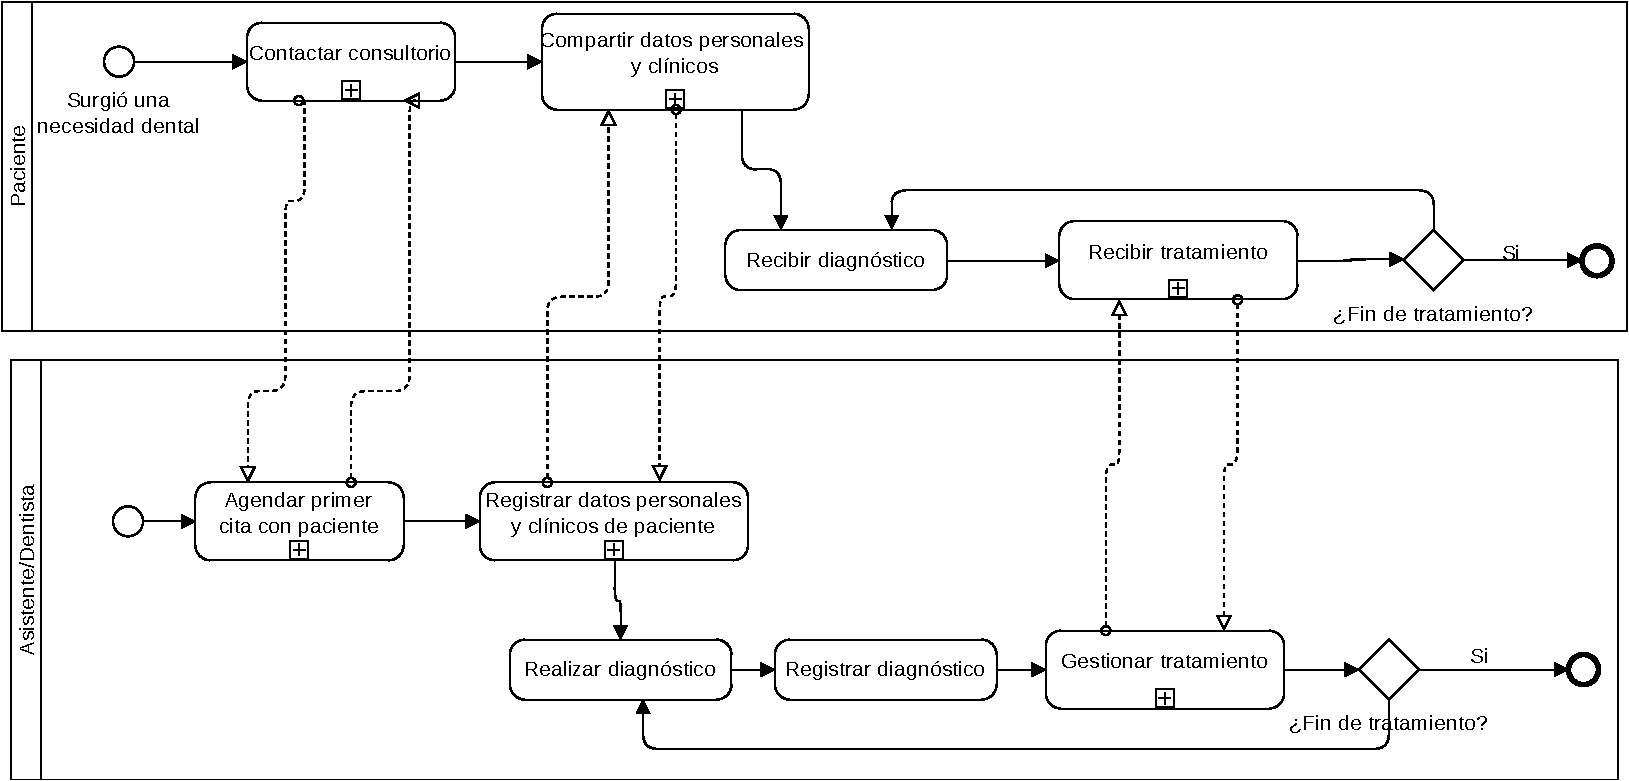
\includegraphics[width=18.5cm, keepaspectratio]{pictures/picture05.pdf}}
\caption{Proceso general actual de tratamiento odontológico}
\end{figure}

\noindent\textbf{Subproceso para contactar consultorio:} Este subproceso se refiere al primer contacto con el consultorio, la forma en que se proporciona la información para la comunicación con el consultorio puede ser a través de una recomendación de otro paciente, por medios de publicidad, o por relación/contacto directo con el personal del consultorio. En caso de que la petición de cita sea aceptada se le confirma la fecha de la cita al paciente.

\begin{figure}[H]
\centering
\centerline{ 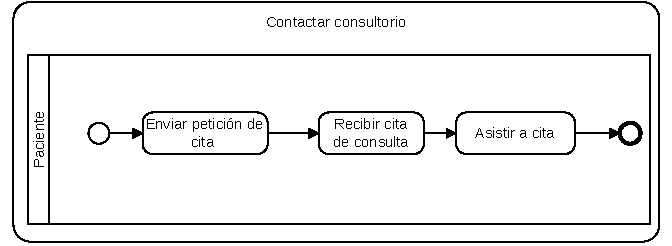
\includegraphics[width=12cm, keepaspectratio]{pictures/picture04.pdf}}
\caption{Subproceso para contactar consultorio}
\end{figure}

\noindent\textbf{Subproceso para compartir datos personales y clínicos:} Este subproceso se refiere a la forma en que se comparten los datos personales, aceptando el aviso de privacidad respectivo, después se pueden identificar dos tipos de datos a registrar independientemente del formato físico o digital, los datos personales del paciente, y los datos clínicos, que incluyen autorización de ingreso, exploración bucal, registro de alergias y el resto de datos sobre el estado de salud del paciente en general, y en específico de la condición bucal.


\begin{figure}[H]
\centering
\centerline{ 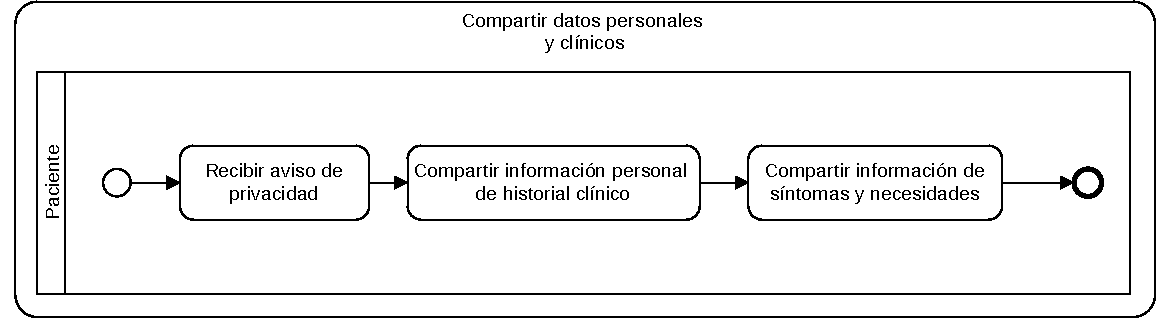
\includegraphics[width=12cm, keepaspectratio]{pictures/picture06.pdf}}
\caption{Subproceso para compartir datos personales y clínicos}
\end{figure}

\noindent\textbf{Subproceso para recibir tratamiento:} Este subproceso se refiere a un ciclo que usualmente se repite hasta que el paciente se encuentra satisfecho con el resultado del tratamiento, o simplemente desea concluirlo en momento determinado. En la cita programada idealmente se realiza un procedimiento de una sola sesión, sin embargo después realizar el procedimiento se puede volver a valorar el estado del tratamiento para hacerle cambios, continuar con el mismo o programar una cita de solo seguimiento. 

\begin{figure}[H]
\centering
\centerline{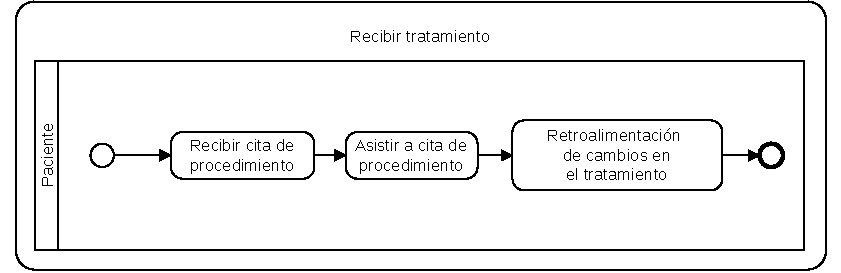
\includegraphics[width=12cm, keepaspectratio]{pictures/picture07.pdf}}
\caption{Subproceso para recibir tratamiento}
\end{figure}

\noindent\textbf{Subproceso para agendar cita con paciente:} Por parte del consultorio, es decir del asistente, del odontólogo o de un administrador que a su vez sea odontólogo, se evalúan las peticiones de los posibles pacientes para determinar si agendar una cita para registrar los datos personales y clínicos respectivos, y valorar el estado del paciente con mayor detalle, y así brindar un diagnóstico. Sin embargo por diferentes motivos es posible que el consultorio rechace la petición inicial de un supuesto cliente/paciente potencial.

\begin{figure}[H]
\centering
\centerline{ 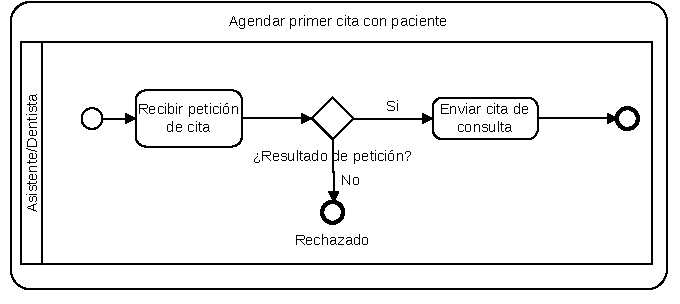
\includegraphics[width=12cm, keepaspectratio]{pictures/picture08.pdf}}
\caption{Subproceso para agendar cita con paciente}
\end{figure}

\noindent\textbf{Subproceso para registrar datos personales y clínicos de paciente:} Este subproceso se refiere al registro de los datos personales y clínicos de los pacientes que realiza el asistente, el odontólogo o el administrador odontólogo, de forma estricta quien captura los datos clínicos es el personal del consultorio, sin embargo para los datos personales, estos pueden ser llenados en formatos preestablecidos por el consultorio por el paciente, siempre verificando después la información. El registro del odontograma es la parte central de registro clínico dental, pues la evolución del paciente, no es más que una secuencia de odontogramas que varían a lo largo del tiempo como consecuencia de los tratamientos a los que se somete el paciente.

\begin{figure}[H]
\centering
\centerline{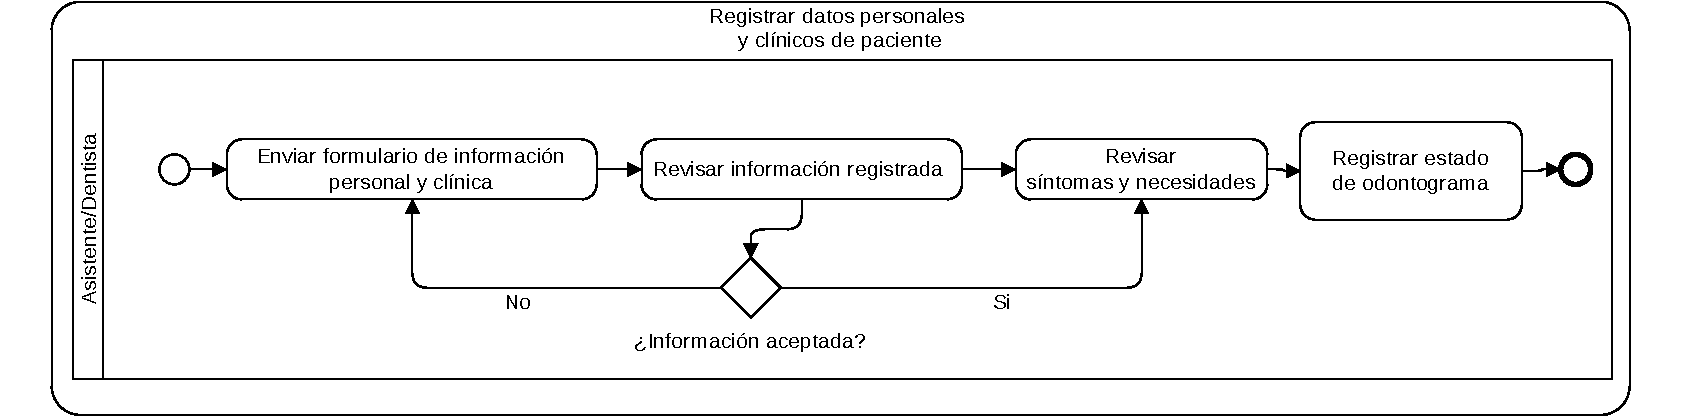
\includegraphics[width=18cm, keepaspectratio]{pictures/picture09.pdf}}
\caption{Subproceso para registrar datos personales y clínicos de paciente}
\end{figure}

\noindent\textbf{Subproceso para gestionar tratamiento:} Este subproceso se refiere a las acciones de registrar, organizar, planificar, citas y procedimientos de los pacientes. El presupuesto evoluciona junto con el tratamiento, y el tratamiento cambia el estado del odontograma al realizar cada procedimiento dental.

\begin{figure}[H]
\centering
\centerline{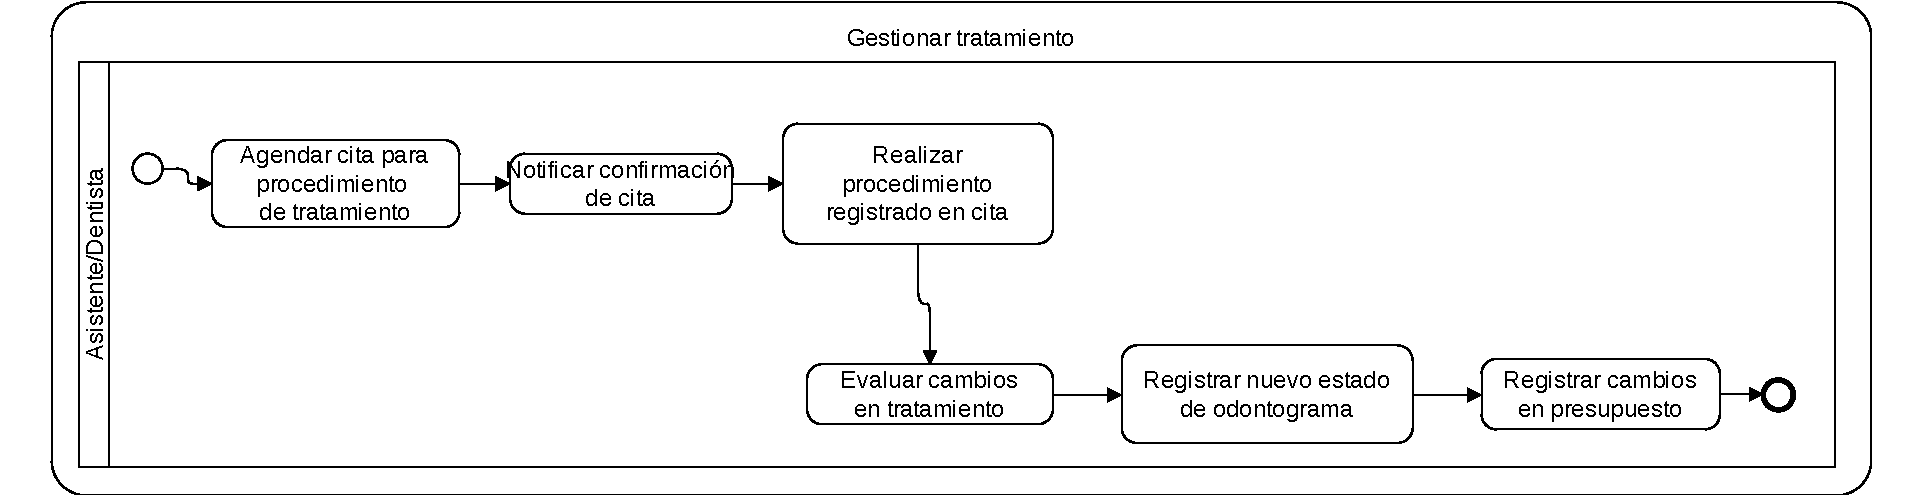
\includegraphics[width=\textwidth, keepaspectratio]{pictures/picture10.pdf}}
\caption{Subproceso para gestionar tratamiento}
\end{figure}

\subsubsection{Modelo propuesto}

\noindent\textbf{Proceso general propuesto de tratamiento odontológico:} Este proceso contempla las partes del proceso actual donde se puede hacer uso de la herramienta dental propuesta.

\begin{figure}[H]
\centering
\centerline{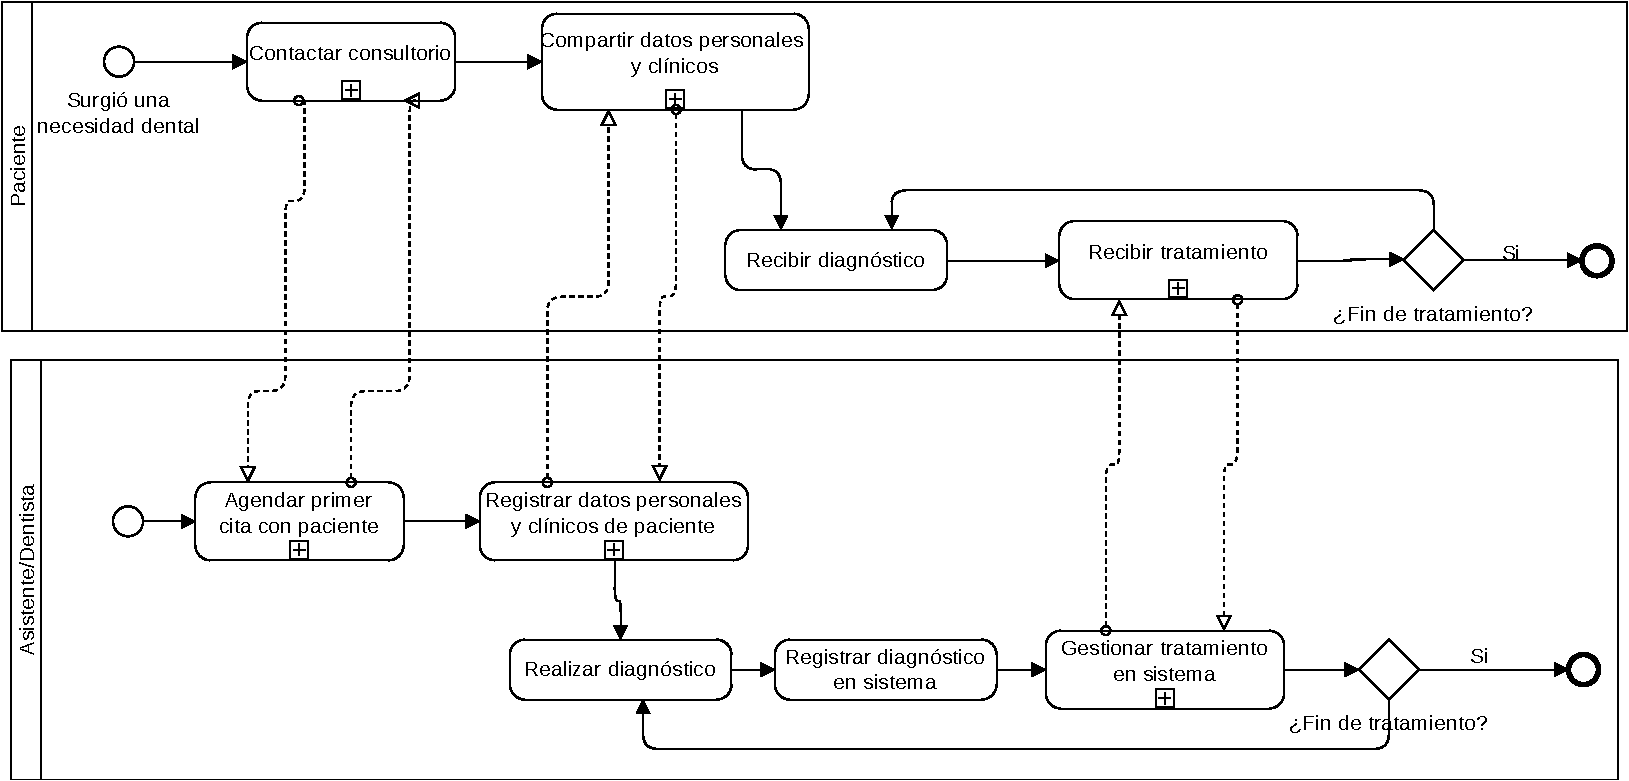
\includegraphics[width=18.5cm, keepaspectratio]{pictures/picture11.pdf}}
\caption{Proceso general propuesto de tratamiento odontológico}
\end{figure}


\noindent\textbf{Subproceso propuesto para registrar datos personales y clínicos de paciente:} Este subproceso se refiere a la parte del proceso general en la cuál la herramienta registra la información del paciente, se deberían poder registrar lo datos personales del paciente, accediendo al sistema para que lo haga el mismo paciente, o el personal del consultorio, esto ya libera tiempo del personal porque no tiene que capturar todos los datos personales, sino que el paciente lo hace, y para los datos clínicos, si es necesario que los capture el personal del consultorio, el registro de los síntomas, el estado del odontograma, el registro del tratamiento, y el registro del presupuesto del procedimiento se registran en el sistema.

\begin{figure}[H]
\centering
\centerline{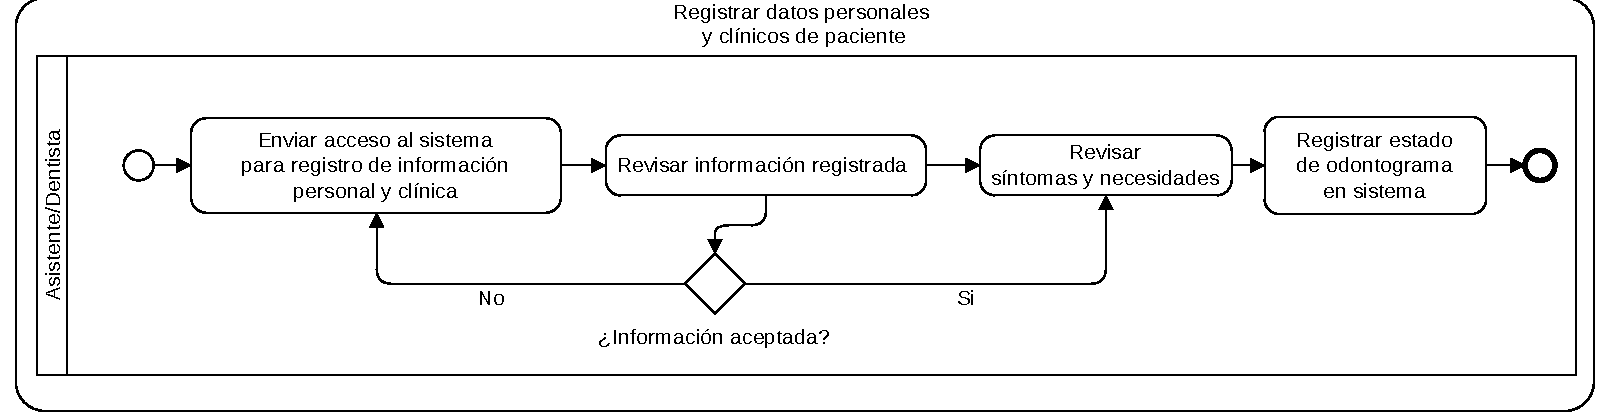
\includegraphics[width=18.5cm, keepaspectratio]{pictures/picture12.pdf}}
\caption{Subproceso propuesto para registrar datos personales y clínicos de paciente}
\end{figure}

\noindent\textbf{Subproceso propuesto para registrar datos personales y clínicos de paciente:} Este subproceso se refiere al registro continuo de procedimientos, citas, presupuestos, pero notificando mediante el sistema las citas a los pacientes, funcionando como recordatorio ya sea en tratamientos tradicionales o simplemente en el seguimiento de pacientes. El paciente es capaz de ver los cambios en el presupuesto de su tratamiento actual.

\begin{figure}[H]
\centering
\centerline{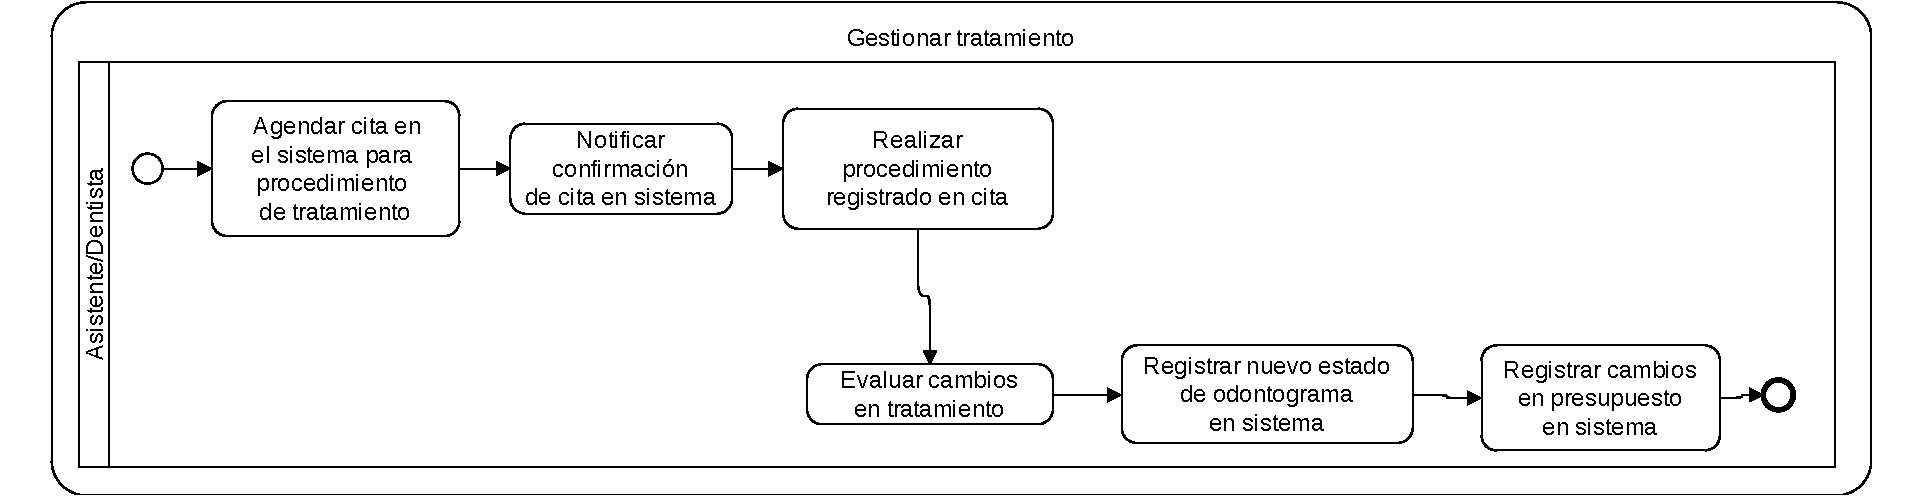
\includegraphics[width=18.5cm, keepaspectratio]{pictures/picture13.pdf}}
\caption{Subproceso propuesto para gestionar tratamiento}
\end{figure}

\newpage
\subsection{Metodología}

Para poder llegar a la construcción final de un producto de software existen una gran variedad de modelos definidos por la ingeniería de software, los cuales son aplicables dependiendo a las características del proyecto a desarrollar, así como cada uno optimiza el desarrollo del mismo modo dependiendo de su definición\cite{A01}. 

\vspace{1em}

Las metodologías ágiles nos permiten aplicar modelos en los que se tiene una retroalimentación del cliente considerándolo como parte del equipo de desarrollo, uno de estos modelos es el modelo de desarrollo evolutivo (también denominado prototipado evolutivo) el cual se basa en la elaboración de una versión inicial del sistema, la cual es expuesta a comentarios del cliente y es refinada a lo largo de diferentes versiones hasta llegar al sistema final. Este modelo considera las actividades de especificación, desarrollo y validación, las cuales se relacionan para poder generar un prototipo a partir de especificaciones generales e ir modificando hasta llegar al sistema final\cite{A07}.

\begin{figure}[H]
\centering
\centerline{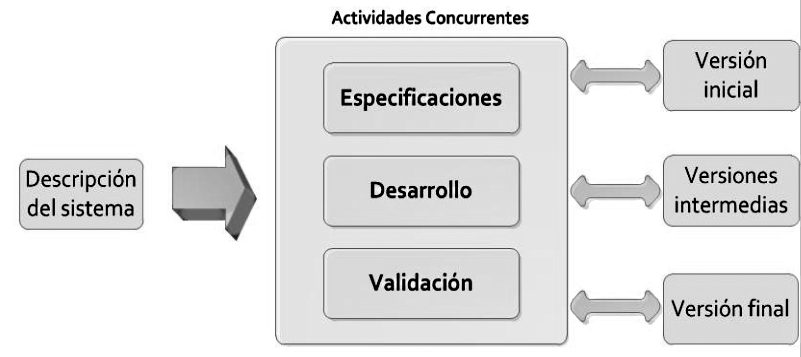
\includegraphics[width=12cm, keepaspectratio]{pictures/picture14.png}}
\caption{Modelo de desarrollo evolutivo}
\end{figure}

\newpage
\subsection{Análisis de requerimientos}

Para poder conocer con detalle la información necesaria para diseñar los diferentes componentes de software que se usarán, se debe partir de los requerimientos básicos del sistema. Los requerimientos para un sistema son descripciones de lo que el sistema debe hacer (en caso de ser construido)\cite{A01}. 

\vspace{1em}

Se puede decir entonces que un requerimiento de software se refiere a la capacidad del sistema necesaria para que el usuario pueda resolver un problema o alcanzar un objetivo, aunque también puede ser una capacidad del software que debe ser reunida o poseída por el sistema o componente del sistema para satisfacer un contrato, especificación, estándar, u otra documentación formal. Para la mayoría de los sistemas grandes, todavía se presenta una fase de ingeniería de requerimientos claramente identificable, antes de comenzar la implementación del sistema\cite{A01}. A continuación se muestra el análisis correspondiente para la obtención de los requerimientos de la herramienta, comenzando por la definición de los actores participantes y luego mostrando el listado de los requerimientos.

\begin{outline}
\1 Id: Identificador del requerimiento
\1 Nombre: Titulo representativo del requerimiento.
\1 Descripción: Explicación del requerimiento.
\end{outline}

\subsubsection{Definición de actores}

En la presente sección se realiza la especificación de los actores que tendrán interacción con la herramienta junto con las actividades que desarrollan.

\begin{itemize}
\item \textbf{Administrador del sistema:} Representa el rol de un usuario predeterminado en el sistema, debe existir por lo menos una instancia de este rol, ya que el es el encargado de dar de alta a todos los otros tipos de usuarios, tiene mayor control sobre los usuarios odontólogo administrador, asistente, odontólogo y paciente, sin embargo no puede modificar el tratamiento ni datos clínicos de un paciente, solo altas, bajas, cambios y consultas de otros usuarios. Puede crear a otros usuarios del tipo administrador, eliminarlos, cambiar sus datos personales, nombres de usuario y contraseñas, pero siempre debe existir por lo menos una instancia.
                
\item \textbf{Administrador odontólogo:} Representa el rol de un usuario con todos los permisos de un Administrador del sistema, pero además puede dar consultar, modificar, y eliminar los datos clínicos de los pacientes. La razón por la cuál existe este actor con nivel de permisos entre un administrador del sistema y un odontólogo es que algunos odontólogos no cuentan con personal de apoyo en el área de sistemas, por lo que todas las acciones de gestión de expedientes, y alta de asistentes, las debe poder realizar el mismo.
                 
\item \textbf{Odontólogo:} Representa el rol de un odontólogo, en un consultorio puede haber más de un odontólogo, en algunos casos dentro del grupo de odontólogos hay jefes o dueños del consultorio, estos odontólogos pudieran asumir el rol de administradores odontólogos. Este actor puede dar de alta pacientes y modificar sus datos tanto personales como clínicos, y también puede dar de alta asistentes.
                 
\item \textbf{Asistente:} Representa el rol de un asistente de un consultorio dental, en ocasiones dado el número de pacientes, y por cuestiones de apoyo en la ejecución de los procedimientos dentales, muchos odontólogos tienen a su cargo asistentes que desempeñan principalmente las tareas de captura, y modificación de datos personales y clínicos de los pacientes, este actor cuenta con esos permisos, sin embargo no puede dar de alta otros asistentes, solo pacientes, esta es una medida que puede variar de consultorio en consultorio pero para efectos del trabajo presente se considera esta situación en la que solo el odontólogo puede dar de alta asistentes.

\item \textbf{Paciente:} Representa el rol de un paciente que asiste al consultorio para realizar consultas diagnósticas, tratamientos, presupuestos.
\end{itemize}

\subsubsection{Requerimientos funcionales}

Los requerimientos funcionales que se consideran respecto a la gestión del tratamiento clínico dental son:

\vspace{1em}

\noindent Id:  \textbf{RF01}\\
Nombre: Registro de pacientes\\
Descripción: La herramienta debe dar la capacidad a los usuarios seleccionados con tal permiso dar de alta un paciente deberá poder dar de alta los datos personales y clínicos del paciente.

\vspace{1em}

\noindent Id:  \textbf{RF02}\\
Nombre: Baja de pacientes\\
Descripción:La herramienta debe dar la capacidad a los usuarios seleccionados con tal permiso de eliminar el historial clínico (datos personales y datos clínicos) de un paciente. Al eliminar un paciente se eliminar toda información asociada a el.

\vspace{1em}

\noindent Id:  \textbf{RF03}\\
Nombre: Actualización de datos de pacientes\\
Descripción: La herramienta debe dar la capacidad a los usuarios seleccionados con tal permiso de modificar tanto los datos personales del paciente, como los datos del historial clínico.

\vspace{1em}

\noindent Id:  \textbf{RF04}\\
Nombre: Consulta de pacientes\\
Descripción: La herramienta debe dar la capacidad a los usuarios seleccionados con tal permiso de buscar a un paciente, para verificar si existe un historial clínico relacionado.

\vspace{1em}

\noindent Id:  \textbf{RF05}\\
Nombre: Generación Reportes\\
Descripción: El sistema ofrecerá al usuario la posibilidad de generar un reporte que contenga los datos considerados en la
norma mexicana NOM-024-SSA3-2012 de Sistemas de información de registro electrónico para la salud, intercambio de información en salud, limitandose al catálogo de datos.

\vspace{1em}

\noindent Id:  \textbf{RF06}\\
Nombre: Notificaciones y recordatorios\\
Descripción: Se deberá poder notificar sobre las citas a los pacientes, mediante correos electrónicos o recordatorios en su teléfono móvil inteligente.

\vspace{1em}

\noindent Id:  \textbf{RF07}\\
Nombre: Registro de tratamientos\\
Descripción: La herramienta debe dar la capacidad a los usuarios que posean el permiso correspondiente, de registrar tratamientos a al expediente de los pacientes.

\vspace{1em}

\noindent Id:  \textbf{RF08}\\
Nombre: Eliminar tratamiento\\
Descripción:La herramienta debe dar la capacidad a los usuarios que posean el permiso correspondiente, de eliminar un tratamiento asignado a un paciente.

\vspace{1em}

\noindent Id:  \textbf{RF09}\\
Nombre: Actualización de tratamiento\\
Descripción: La herramienta debe dar la capacidad a los usuarios que posean el permiso correspondiente, de del tratamiento del paciente como procedimientos relacionados con el tratamiento.

\vspace{1em}


\noindent Id:  \textbf{RF10}\\
Nombre: Registro de diagnósticos\\
Descripción: La herramienta debe dar la capacidad a los usuarios que posean el permiso correspondiente, de registrar el estado dental del paciente en un odontograma.

\vspace{1em}

\noindent Id:  \textbf{RF11}\\
Nombre: Eliminación de diagnósticos\\
Descripción:  La herramienta debe dar la capacidad a los usuarios que posean el permiso correspondiente, de eliminar los odontogramas relacionados al expediente de los pacientes.

\vspace{1em}

\noindent Id:  \textbf{RF12}\\
Nombre: Actualización de diagnósticos\\
Descripción: La herramienta debe dar la capacidad a los usuarios que posean el permiso correspondiente, de modificar el estado del odontograma actual o el último registrado.

\vspace{1em}

\noindent Id:  \textbf{RF13}\\
Nombre: Registro de citas\\
Descripción: La herramienta debe dar la capacidad a los usuarios que posean el permiso correspondiente, de registrar en una agenda o calendario las citas de los pacientes del odontólogo.

\vspace{1em}

\noindent Id:  \textbf{RF14}\\
Nombre: Eliminar citas\\
Descripción: o de citas\\
Descripción: La herramienta debe dar la capacidad a los usuarios que posean el permiso correspondiente, de eliminar las citas de los pacientes en la agenda o calendario del odontólogo.

\vspace{1em}

\noindent Id:  \textbf{RF15}\\
Nombre: Actualización de citas\\
Descripción: La herramienta debe dar la capacidad a los usuarios que posean el permiso correspondiente, de modificar la fecha y detalles de las citas de los pacientes en la agenda o calendario del odontólogo.


\noindent Id:  \textbf{RF16}\\
Nombre: Consulta de citas\\
Descripción: La herramienta debe dar la capacidad a los usuarios que posean el permiso correspondiente, de consultar las citas asignadas a un odontólogo.

\vspace{1em}

\noindent Id: \textbf{RF17}\\
Nombre: Bitácora de actividad en sistema\\
Descripción: Toda creación, modificación, destrucción de información en el sistema debe ser registrado en una bitácora, que guardará la clave del usuario que hizo la transacción.

\vspace{1em}

\noindent Id: \textbf{RF18}\\
Nombre: Autenticación de usuarios\\
Descripción: El sistema debe autenticar a los usuarios que utilizarán el sistema, y cargará el perfil operacional su tipo de usuario respectivo.


\vspace{1em}

\noindent Id: \textbf{RF19}\\
Nombre: Respaldo de datos\\
Descripción: El sistema debe proveer un mecanismo interno o externo ya sea conexión a servicios, ejecución de programa, scripts de sistema, o cualquier otro método viable para respaldar la información de los registros clínicos y datos personales de los pacientes.

\vspace{1em}

\noindent Id: \textbf{RF20}\\
Nombre: Gestión de presupuesto del tratamiento\\
Descripción: La herramienta debe dar la capacidad a los usuarios que posean el permiso correspondiente de registrar y modificar, el presupuesto asociado a los tratamientos de los pacientes, sin embargo la modificación será manual, no automática, el paciente solo visualizara el estado actual del presupuesto de su tratamiento.  

\newpage





\section{Diseño de arquitectura de software}

\subsection{Casos de uso del módulo}








\section{Diseño de la arquitectura de software}


\subsection{Vista de escenarios}

La descripción de la arquitectura se ilustra utilizando un conjunto de casos de uso, o escenarios lo que genera una quinta vista. Los escenarios describen secuencias de interacciones entre objetos, y entre procesos. 



\subsubsection{Casos de uso de Administrador del sistema}

La figura que se presenta a continuación. muestra el diagrama de los casos de uso correspondientes al actor Administrador del sistema.

\begin{figure}[H]
\centering
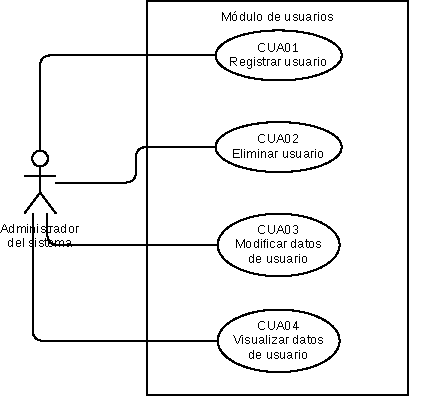
\includegraphics[width=10cm, keepaspectratio]{pictures/picture25.pdf}
\caption{Diagrama de casos de uso del actor Administrador del sistema}
\end{figure}

\begin{longtable}[H]{|p{0.25\textwidth}|p{12cm}|}
\hline\textbf{Id}         & \textbf{CUA01}\\ \hline
\textbf{Nombre:}          & Registrar usuario           \\ \hline
\textbf{Actor:}           & Administrador del sistema   \\ \hline
\textbf{Objetivo:}        & Permitir al Administrador registrar a un nuevo usuario. \\ \hline
\textbf{Precondiciones:}  & 
\begin{minipage}[t]{\linewidth}
\begin{itemize}[nosep]
\item El usuario a registrar no debe estar registrado previamente en la herramienta.
\end{itemize}
\vspace{0.3em}
\end{minipage}\\ \hline
\textbf{Postcondiciones:} & 
\begin{minipage}[t]{\linewidth}
\begin{itemize}[nosep]
\item Se registrará en la herramienta un nuevo paciente.
\item  Se actualizará el listado de usuarios.
\end{itemize}
\vspace{0.2em}
\end{minipage}\\ \hline
\textbf{Errores:}         & 
\begin{minipage}[t]{\linewidth}
\begin{itemize}[nosep]
\item Muestra el mensaje de error ``Falta un dato obligatorio para efectuar la operación solicitada.''
\item Se muestra una pantalla con el mensaje de error ``Tipo de dato incorrecto.''
\end{itemize}
\vspace{0.2em}
\end{minipage}\\ \hline
\caption{Especificación de caso de uso Registrar usuario del actor Administrador del sistema.}
\label{table:1}
\end{longtable}

\textbf{Trayectoria base:}    
\begin{enumerate}
\item \includegraphics[height=1em]{pictures/picture22.png} Solicita registrar un nuevo usuario.
\item \includegraphics[height=1em]{pictures/picture23.png} Solicita el nombre de usuario y contraseña, y el tipo de usuario.
\item \includegraphics[height=1em]{pictures/picture22.png} Ingresa los datos del usuario a registrar.
\item \includegraphics[height=1em]{pictures/picture23.png} Verifica que se hayan ingresado valores en el campo de texto.
\item \includegraphics[height=1em]{pictures/picture23.png} Verifica que los valores ingresados tengan el tipo correcto.
\item \includegraphics[height=1em]{pictures/picture23.png} Registra al usuario nuevo en la base de datos.
\end{enumerate}
\textbf{Trayectoria alternativa:}  \\
\vspace{1em}
{\large Trayectoria alternativa A \par}
\textbf{Condición:} El usuario no ingresó valores en el campo de texto, los dejó vacios.
\begin{enumerate}
\item \includegraphics[height=1em]{pictures/picture23.png} Muestra en la pantalla con el mensaje de error ``Falta un dato obligatorio para efectuar la operación solicitada.''
\item \includegraphics[height=1em]{pictures/picture23.png} Continúa con el paso 3 de la trayectoria principal.
\end{enumerate}
{\large Trayectoria alternativa B \par}
\vspace{0.3em}
\textbf{Condición:} El usuario no ingresó valores de tipo incorrecto.
\begin{enumerate}
\item \includegraphics[height=1em]{pictures/picture23.png} Muestra en la pantalla el error ``Formato incorrecto``.
\item \includegraphics[height=1em]{pictures/picture23.png} Continúa con el paso 3 de la trayectoria principal.
\end{enumerate}

\begin{longtable}[H]{|p{0.25\textwidth}|p{12cm}|}
\hline\textbf{Id}         & \textbf{CUA02}           \\ \hline
\textbf{Nombre:}          & Eliminar usuario         \\ \hline
\textbf{Actor:}           & Administrador del sistema\\ \hline
\textbf{Objetivo:}        & Permitir al Administrador del sistema eliminar a otro usuario en la herramienta. \\ \hline
\textbf{Precondiciones:}  &            
\begin{minipage}[t]{\linewidth}
\begin{itemize}[nosep]
\item El usuario a eliminar debe estar registrado en el sistema.
\end{itemize}
\vspace{0.3em}
\end{minipage}\\ \hline
\textbf{Postcondiciones:} & \begin{minipage}[t]{\linewidth}        
\begin{itemize}[nosep]
\item Se eliminará de la herramienta toda la información del usuario..
\item Se actualizará el listado de usuarios.
\end{itemize}
\vspace{0.2em}
\end{minipage}\\ \hline
\textbf{Errores:}         & \begin{minipage}[t]{\linewidth}        
\begin{itemize}[nosep]
\item Se muestra en pantalla el mensaje de error ``No puede eliminar su propia cuenta siendo usuario administador'', cuando el usuario intente borrar su propia cuenta.
\end{itemize}
\vspace{0.2em}
\end{minipage}\\ \hline
\caption{Especificación de caso de uso Eliminar usuario del actor Administrador del sistema.}
\label{table:1}
\end{longtable}

\textbf{Trayectoria base:}            \begin{enumerate}
\item \includegraphics[height=1em]{pictures/picture22.png} Solicita borrar a otro usuario en particular.
\item \includegraphics[height=1em]{pictures/picture23.png} Verifica en caso seleccionar a un usuario tipo administrador que no sea el mismo.
\item \includegraphics[height=1em]{pictures/picture22.png} Solicita confirmación por parte del usuario para realizar la acción.
\item \includegraphics[height=1em]{pictures/picture22.png} Confirma la solicitud mostrada.
\end{enumerate}
\textbf{Trayectoria alternativa:}  Ninguna            

\begin{longtable}[H]{|p{0.25\textwidth}|p{12cm}|}
\hline\textbf{Id}         & \textbf{CUA03}   \\ \hline
\textbf{Nombre:}          & Modificar datos de usuario     \\ \hline
\textbf{Actor:}           & Administrador del sistema      \\ \hline
\textbf{Objetivo:}        & Permitir al Administrador del sistema modificar los datos personales de otro, pero no los clínicos. \\ \hline
\textbf{Precondiciones:}  &    
\begin{minipage}[t]{\linewidth}
\begin{itemize}[nosep]
\item El usuario a el cuál se pretende modificar su información debe estar registrado en el sistema.
\end{itemize}
\vspace{0.3em}
\end{minipage}\\ \hline
\textbf{Postcondiciones:} & \begin{minipage}[t]{\linewidth}
\begin{itemize}[nosep]
\item Actualización de información de usuario en la base de datos de la herramienta.
\end{itemize}
\vspace{0.2em}
\end{minipage}\\ \hline

\textbf{Errores:}         & \begin{minipage}[t]{\linewidth}
\begin{itemize}[nosep]
\item Muestra el mensaje de error ``Falta un dato obligatorio para efectuar la operación solicitada.''
\item Se muestra una pantalla con el mensaje de error ``El tipo de dato no es correcto.''
\end{itemize}
\vspace{0.2em}
\end{minipage}\\ \hline
\caption{Especificación de caso de uso Modificar datos de usuario del actor Administrador del sistema.}
\label{table:1}
\end{longtable}

\textbf{Trayectoria base:}        \begin{enumerate}
\item \includegraphics[height=1em]{pictures/picture22.png} Solicita modificar los datos de otro usuario en particular.
\item \includegraphics[height=1em]{pictures/picture23.png} Muestra el formulario para cambiar los datos del usuario.
\item \includegraphics[height=1em]{pictures/picture22.png} Realiza el llenado o modificación de los datos.
\item \includegraphics[height=1em]{pictures/picture23.png} Verifica que los cambias realizados cumplan con las condiciones de formato correcto.
\item \includegraphics[height=1em]{pictures/picture22.png} Verifica que los cambias realizados cumplan con las condiciones de tipo correcto.
\item \includegraphics[height=1em]{pictures/picture22.png} Verifica que alguno de los campos establecidos como no vacíos (obligatorio llenar), se encuentre sin información tras la modificación.
cambias realizados cumplan con las condiciones de tipo correcto.
\item \includegraphics[height=1em]{pictures/picture22.png} Solicita confirmar la modificación.
\item \includegraphics[height=1em]{pictures/picture22.png} Acepta la confirmación.
\end{enumerate}
\textbf{Trayectoria alternativa:} 
{\large Trayectoria alternativa A \par}
\vspace{0.3em}
\textbf{Condición:} El usuario no acepto la confirmación de modificación.
\begin{enumerate}
\item \includegraphics[height=1em]{pictures/picture23.png} Muestra la pantalla de modificación de datos del usuario nuevamente.
\item \includegraphics[height=1em]{pictures/picture23.png} Continúa con el paso 2 de la trayectoria principal.
\end{enumerate}

\begin{longtable}[H]{|p{0.25\textwidth}|p{12cm}|}
\hline\textbf{Id}         & \textbf{CUA04}     \\ \hline
\textbf{Nombre:}          & Visualizar datos de usuario      \\ \hline
\textbf{Actor:}           & Administrador del sistema        \\ \hline
\textbf{Objetivo:}        & Permitir al Administrador del sistema visualizar los datos de un usuario en específico. \\ \hline
\textbf{Precondiciones:}  &      
\begin{minipage}[t]{\linewidth}
\begin{itemize}[nosep]
\item El usuario a el cuál se pretende visualizar debe estar registrado en el sistema.
\end{itemize}
\vspace{0.3em}
\end{minipage}\\ \hline
\textbf{Postcondiciones:} & \begin{minipage}[t]{\linewidth}  
\begin{itemize}[nosep]
\item Se muestran los datos personales del usuario seleccionado.
\end{itemize}
\vspace{0.2em}
\end{minipage}\\ \hline
\textbf{Errores:}         & Ninguno            \\ \hline
\caption{Especificación de caso de uso Visualizar datos de usuario del actor Administrador del sistema.}
\label{table:1}
\end{longtable}
\textbf{Trayectoria base:}     \begin{enumerate}
\item \includegraphics[height=1em]{pictures/picture22.png} Solicita ver el listado de usuarios.
\item \includegraphics[height=1em]{pictures/picture23.png} Muestra el lista de usuarios de todos los tipos (Administrador, Odontólogo administrador, Asistentes y Pacientes).
\item \includegraphics[height=1em]{pictures/picture22.png} Selecciona uno de los usuarios.
\item \includegraphics[height=1em]{pictures/picture23.png} Muestra los datos personales de ese usuario.
\end{enumerate}
\textbf{Trayectoria alternativa:} Ninguna

\newpage
\subsubsection{Casos de uso de Odontólogo administrador}

La figura que se presenta a continuación. muestra el diagrama de los casos de uso correspondientes al actor Odontólogo administrador.

\begin{figure}[H]
\centering
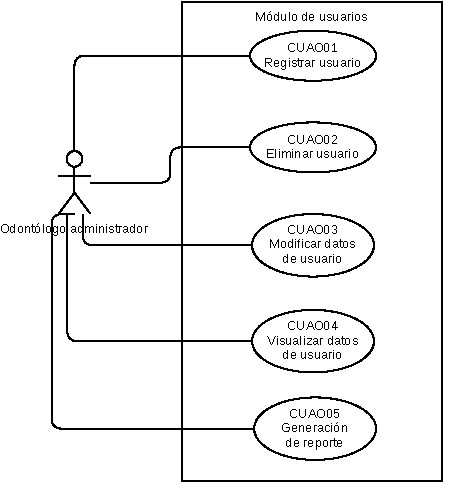
\includegraphics[width=10cm, keepaspectratio]{pictures/picture26.pdf}
\caption{Diagrama de casos de uso del actor Odontólogo administrador}
\end{figure}

\begin{longtable}[H]{|p{0.25\textwidth}|p{12cm}|}
\hline\textbf{Id}         & \textbf{CUAO01}             \\ \hline
\textbf{Nombre:}          & Registrar usuario           \\ \hline
\textbf{Actor:}           & Administrador odontólogo   \\ \hline
\textbf{Objetivo:}        & Permitir al Administrador registrar a un nuevo usuario. \\ \hline
\textbf{Precondiciones:}  & 
\begin{minipage}[t]{\linewidth}
\begin{itemize}[nosep]
\item El usuario a registrar no debe estar registrado previamente en la herramienta.
\end{itemize}
\vspace{0.3em}
\end{minipage}\\ \hline
\textbf{Postcondiciones:} & 
\begin{minipage}[t]{\linewidth}
\begin{itemize}[nosep]
\item Se registrará en la herramienta un nuevo paciente.
\item  Se actualizará el listado de usuarios.
\end{itemize}
\vspace{0.2em}
\end{minipage}\\ \hline

\textbf{Errores:}         & 
\begin{minipage}[t]{\linewidth}
\begin{itemize}[nosep]
\item Muestra el mensaje de error ``Falta un dato obligatorio para efectuar la operación solicitada.''
\item Se muestra una pantalla con el mensaje de error ``Tipo de dato incorrecto.''
\end{itemize}
\vspace{0.2em}
\end{minipage}\\ \hline
\caption{Especificación de caso de uso Registrar usuario del actor Administrador odontólogo .}
\label{table:1}
\end{longtable}
\textbf{Trayectoria base:}
\begin{enumerate}
\item \includegraphics[height=1em]{pictures/picture22.png} Solicita registrar un nuevo usuario.
\item \includegraphics[height=1em]{pictures/picture23.png} Solicita el nombre de usuario y contraseña, y el tipo de usuario.
\item \includegraphics[height=1em]{pictures/picture22.png} Ingresa los datos del usuario a registrar.
\item \includegraphics[height=1em]{pictures/picture23.png} Verifica que se hayan ingresado valores en el campo de texto.
\item \includegraphics[height=1em]{pictures/picture23.png} Verifica que los valores ingresados tengan el tipo correcto.
\item \includegraphics[height=1em]{pictures/picture23.png} Registra al usuario nuevo en la base de datos.
\end{enumerate}
\textbf{Trayectoria alternativa:} 

{\large Trayectoria alternativa A \par}
\vspace{0.3em}
\textbf{Condición:} El usuario no ingresó valores en el campo de texto, los dejó vacios.
\begin{enumerate}
\item \includegraphics[height=1em]{pictures/picture23.png} Muestra en la pantalla con el mensaje de error ``Falta un dato obligatorio para efectuar la operación solicitada.''
\item \includegraphics[height=1em]{pictures/picture23.png} Continúa con el paso 3 de la trayectoria principal.
\end{enumerate}
{\large Trayectoria alternativa B \par}
\vspace{0.3em}
\textbf{Condición:} El usuario no ingresó valores de tipo incorrecto.
\begin{enumerate}
\item \includegraphics[height=1em]{pictures/picture23.png} Muestra en la pantalla el error ``Formato incorrecto``.
\item \includegraphics[height=1em]{pictures/picture23.png} Continúa con el paso 3 de la trayectoria principal.
\end{enumerate}

\begin{longtable}[H]{|p{0.25\textwidth}|p{12cm}|}
\hline\textbf{Id}         & \textbf{CUAO02}           \\ \hline
\textbf{Nombre:}          & Eliminar usuario          \\ \hline
\textbf{Actor:}           & Administrador odontólogo \\ \hline
\textbf{Objetivo:}        & Permitir al Administrador odontólogo  eliminar a otro usuario en la herramienta. \\ \hline
\textbf{Precondiciones:}  &             
\begin{minipage}[t]{\linewidth}
\begin{itemize}[nosep]
\item El usuario a eliminar debe estar registrado en el sistema.
\end{itemize}
\vspace{0.3em}
\end{minipage}\\ \hline
\textbf{Postcondiciones:} & \begin{minipage}[t]{\linewidth}         
\begin{itemize}[nosep]
\item Se eliminará de la herramienta toda la información del usuario..
\item Se actualizará el listado de usuarios.
\end{itemize}
\vspace{0.2em}
\end{minipage}\\ \hline

\textbf{Errores:}         & \begin{minipage}[t]{\linewidth}         
\begin{itemize}[nosep]
\item Se muestra en pantalla el mensaje de error ``No puede eliminar su propia cuenta siendo usuario administador'', CUAOndo el usuario intente borrar su propia cuenta.
\end{itemize}
\vspace{0.2em}
\end{minipage}\\ \hline
\caption{Especificación de caso de uso Eliminar usuario del actor Administrador odontólogo .}
\label{table:1}
\end{longtable}

\textbf{Trayectoria base:}       \begin{enumerate}
\item \includegraphics[height=1em]{pictures/picture22.png} Solicita borrar a otro usuario en particular.
\item \includegraphics[height=1em]{pictures/picture23.png} Verifica en caso seleccionar a un usuario tipo administrador que no sea el mismo.
\item \includegraphics[height=1em]{pictures/picture23.png} Solicita confirmación por parte del usuario para realizar la acción.
\item \includegraphics[height=1em]{pictures/picture22.png} Confirma la solicitud mostrada.
\end{enumerate}
\textbf{Trayectoria alternativa:}  Ninguna         

\begin{longtable}[H]{|p{0.25\textwidth}|p{12cm}|}
\hline\textbf{Id}   & \textbf{CUAO03}   \\ \hline
\textbf{Nombre:}    & Modificar datos de usuario      \\ \hline
\textbf{Actor:}     & Administrador odontólogo       \\ \hline
\textbf{Objetivo:}  & Permitir al Administrador odontólogo  modificar los datos personales de otro, pero no los clínicos. \\ \hline
\textbf{Precondiciones:}          &     
\begin{minipage}[t]{\linewidth}
\begin{itemize}[nosep]
\item El usuario a el cuál se pretende modificar su información debe estar registrado en el sistema.
\end{itemize}
\vspace{0.3em}
\end{minipage}\\ \hline
\textbf{Postcondiciones:}         & \begin{minipage}[t]{\linewidth} 
\begin{itemize}[nosep]
\item Actualización de información de usuario en la base de datos de la herramienta.
\end{itemize}
\vspace{0.2em}
\end{minipage}\\ \hline

\textbf{Errores:}   & \begin{minipage}[t]{\linewidth} 
\begin{itemize}[nosep]
\item Muestra el mensaje de error ``Falta un dato obligatorio para efectuar la operación solicitada.''
\item Se muestra una pantalla con el mensaje de error ``El tipo de dato no es correcto.''
\end{itemize}
\vspace{0.2em}
\end{minipage}\\ \hline
\caption{Especificación de caso de uso Modificar datos de usuario del actor Administrador odontólogo .}
\label{table:1}
\end{longtable}
\textbf{Trayectoria base:}
\begin{enumerate} 
\item \includegraphics[height=1em]{pictures/picture22.png} Solicita modificar los datos de otro usuario en particular.
\item \includegraphics[height=1em]{pictures/picture23.png} Muestra el formulario para cambiar los datos del usuario.
\item \includegraphics[height=1em]{pictures/picture22.png} Realiza el llenado o modificación de los datos.
\item \includegraphics[height=1em]{pictures/picture23.png} Verifica que los cambias realizados cumplan con las condiciones de formato correcto.
\item \includegraphics[height=1em]{pictures/picture22.png} Verifica que los cambias realizados cumplan con las condiciones de tipo correcto.
\item \includegraphics[height=1em]{pictures/picture22.png} Verifica que alguno de los campos establecidos como no vacíos (obligatorio llenar), se encuentre sin información tras la modificación.
cambias realizados cumplan con las condiciones de tipo correcto.
\item \includegraphics[height=1em]{pictures/picture23.png} Solicita confirmar la modificación.
\item \includegraphics[height=1em]{pictures/picture22.png} Acepta la confirmación.
\end{enumerate}
\textbf{Trayectoria alternativa:}   
{\large Trayectoria alternativa A \par}
\vspace{0.3em}
\textbf{Condición:} El usuario no acepto la confirmación de modificación.
\begin{enumerate}
\item \includegraphics[height=1em]{pictures/picture23.png} Muestra la pantalla de modificación de datos del usuario nuevamente.
\item \includegraphics[height=1em]{pictures/picture23.png} Continúa con el paso 2 de la trayectoria principal.
\end{enumerate}

\begin{longtable}[H]{|p{0.25\textwidth}|p{12cm}|}
\hline\textbf{Id}   & \textbf{CUAO04}     \\ \hline
\textbf{Nombre:}    & Visualizar datos de usuario       \\ \hline
\textbf{Actor:}     & Administrador odontólogo         \\ \hline
\textbf{Objetivo:}  & Permitir al Administrador odontólogo  visualizar los datos de un usuario en específico. \\ \hline
\textbf{Precondiciones:}          &       
\begin{minipage}[t]{\linewidth}
\begin{itemize}[nosep]
\item El usuario a el cuál se pretende visualizar debe estar registrado en el sistema.
\end{itemize}
\vspace{0.3em}
\end{minipage}\\ \hline
\textbf{Postcondiciones:}         & \begin{minipage}[t]{\linewidth}   
\begin{itemize}[nosep]
\item Se muestran los datos personales del usuario seleccionado.
\end{itemize}
\vspace{0.2em}
\end{minipage}\\ \hline

\textbf{Errores:}   & Ninguno             \\ \hline
\caption{Especificación de caso de uso Visualizar datos de usuario del actor Administrador odontólogo .}
\label{table:1}
\end{longtable}





\begin{longtable}[H]{|p{0.25\textwidth}|p{12cm}|}
\hline\textbf{Id}   & \textbf{CUOA05}    \\ \hline
\textbf{Nombre:}    & Generación de reporte           \\ \hline
\textbf{Actor:}     & Odontólogo administrador        \\ \hline
\textbf{Objetivo:}  & Permitir al Odontólogo administrador generar reportes con información de los pacientes \\ \hline
\textbf{Precondiciones:}          &      
\begin{minipage}[t]{\linewidth}
\begin{itemize}[nosep]
\item Los datos del paciente deben haber sido llenado en forma total o parcial, para poder mostrarlos en el reporte.
\end{itemize}
\vspace{0.3em}
\end{minipage}\\ \hline
\textbf{Postcondiciones:}         & \begin{minipage}[t]{\linewidth}  
\begin{itemize}[nosep]
\item Se genera un reporte en formato PDF con los datos clínicos y personales del paciente.
\end{itemize}
\vspace{0.2em}
\end{minipage}\\ \hline
      
\\ \hline
\textbf{Errores:}   &      
-
\\ \hline
\caption{Especificación de caso de uso Generación de reportes de Odontólogo administrador.}
\label{table:1}
\end{longtable}
\textbf{Trayectoria base:}        
\begin{enumerate}  
\item \includegraphics[height=1em]{pictures/picture22.png} Solicita la generación del reporte de un paciente.
\item \includegraphics[height=1em]{pictures/picture23.png} Muestra la pantalla con las opciones de reportes disponibles.
\item \includegraphics[height=1em]{pictures/picture22.png} Selecciona a un reporte.
\item \includegraphics[height=1em]{pictures/picture23.png} Genera el reporte con los datos del paciente.
\end{enumerate}
\textbf{Trayectoria alternativa:} Ninguna  

\begin{longtable}[H]{|p{0.25\textwidth}|p{12cm}|}
\hline\textbf{Id}   & \textbf{CUOA06}             \\ \hline
\textbf{Nombre:}    & Visualizar información de paciente       \\ \hline
\textbf{Actor:}     & Odontólogo administrador   \\ \hline
\textbf{Objetivo:}  & Permitir al Odontólogo administrador visualizar los datos clínicos y personales de un paciente. \\ \hline
\textbf{Precondiciones:}          & 
\begin{minipage}[t]{\linewidth}
\begin{itemize}[nosep]
\item Los datos del paciente deben haber sido llenado en forma total o parcial, para poder mostrarlos en el reporte.
\end{itemize}
\vspace{0.3em}
\end{minipage}\\ \hline
\textbf{Postcondiciones:}         & \begin{minipage}[t]{\linewidth}           
\begin{itemize}[nosep]
\item Se muestran los datos del usuario, su odontograma, sus tratamientos, y su información personal.
\end{itemize}
\vspace{0.2em}
\end{minipage}\\ \hline
\textbf{Errores:}   & 
-
\\ \hline
\caption{Especificación de caso de uso Visualizar información de paciente de Odontólogo administrador.}
\label{table:1}
\end{longtable}
\textbf{Trayectoria base:}        
\begin{enumerate}           
\item \includegraphics[height=1em]{pictures/picture22.png} Solicita la visualización de los datos de un paciente en particular.
\item \includegraphics[height=1em]{pictures/picture23.png} Muestra la pantalla con las opciones a visualizar, entre las cuales está el tratamiento del paciente, odontogramas de la evolución de su tratamiento, el odontograma actual y sus datos personales.
\item \includegraphics[height=1em]{pictures/picture22.png} Selecciona una opción de visualización.
\item \includegraphics[height=1em]{pictures/picture23.png} Muestra la pantalla con los datos solicitados del paciente.
\end{enumerate}
\textbf{Trayectoria alternativa:}  Ninguna       



\begin{longtable}[H]{|p{0.25\textwidth}|p{12cm}|}
\hline\textbf{Id}   & \textbf{CUOA07}        \\ \hline
\textbf{Nombre:}    & Consultar tratamientos de paciente   \\ \hline
\textbf{Actor:}     & Odontólogo administrador            \\ \hline
\textbf{Objetivo:}  & Permitir al Odontólogo administrador consultar el tratamiento de un paciente. \\ \hline
\textbf{Precondiciones:}          &          
\begin{minipage}[t]{\linewidth}
\begin{itemize}[nosep]
\item El paciente debe tener al menos registrado un tratamiento.
\end{itemize}
\vspace{0.3em}
\end{minipage}\\ \hline
\textbf{Postcondiciones:}         & \begin{minipage}[t]{\linewidth}      
\begin{itemize}[nosep]
\item Se muestran los datos del tratamiento, detalles, y procedimientos relacionados al mismo.
\end{itemize}
\vspace{0.2em}
\end{minipage}\\ \hline
\textbf{Errores:}   &          
-
\\ \hline
\caption{Especificación de caso de uso Consultar tratamientos de paciente de Odontólogo administrador.}
\label{table:1}
\end{longtable}

\textbf{Trayectoria base:}        
\begin{enumerate}      
\item \includegraphics[height=1em]{pictures/picture22.png} Solicita la consulta del tratamiento de un paciente.
\item \includegraphics[height=1em]{pictures/picture23.png} Muestra la pantalla con la información del tratamiento solicitada.
\end{enumerate}
\textbf{Trayectoria alternativa:}  Ninguna  

\begin{longtable}[H]{|p{0.25\textwidth}|p{12cm}|}
\hline\textbf{Id}   & \textbf{CUOA08}        \\ \hline
\textbf{Nombre:}    & Registrar diagnóstico de paciente   \\ \hline
\textbf{Actor:}     & Odontólogo administrador            \\ \hline
\textbf{Objetivo:}  & Permitir al Odontólogo administrador consultar el tratamiento de un paciente. \\ \hline
\textbf{Precondiciones:}          &          
\begin{minipage}[t]{\linewidth}
\begin{itemize}[nosep]
\item El paciente debe tener al menos registrado un tratamiento.
\end{itemize}
\vspace{0.3em}
\end{minipage}\\ \hline
\textbf{Postcondiciones:}         & \begin{minipage}[t]{\linewidth}      
\begin{itemize}[nosep]
\item Se muestran los datos del tratamiento, detalles, y procedimientos relacionados al mismo.
\end{itemize}
\vspace{0.2em}
\end{minipage}\\ \hline
\textbf{Errores:}   &          
-
\\ \hline
\caption{Especificación de caso de uso Registrar diagnóstico de paciente de Odontólogo administrador.}
\label{table:1}
\end{longtable}

\textbf{Trayectoria base:}        
\begin{enumerate}   
\item \includegraphics[height=1em]{pictures/picture22.png} Solicita la consulta del tratamiento de un paciente.
\item \includegraphics[height=1em]{pictures/picture23.png} Muestra la pantalla con la información del tratamiento solicitada.
\end{enumerate}
\textbf{Trayectoria alternativa:}  Ninguna  

\subsubsection{Casos de uso de Odontólogo}


\begin{longtable}[H]{|p{0.25\textwidth}|p{12cm}|}
\hline\textbf{Id}   & \textbf{CUO01}             \\ \hline
\textbf{Nombre:}    & Registrar paciente         \\ \hline
\textbf{Actor:}     & Odontólogo  \\ \hline
\textbf{Objetivo:}  & Permitir al Odontólogo registrar a un nuevo paciente. \\ \hline
\textbf{Precondiciones:}          &
\begin{minipage}[t]{\linewidth}
\begin{itemize}[nosep]
\item El paciente a registrar no debe existir en la base de datos de la herramienta.
\end{itemize}
\vspace{0.3em}
\end{minipage}\\ \hline
\textbf{Postcondiciones:}         &
\begin{minipage}[t]{\linewidth}
\begin{itemize}[nosep]
\item Se registrará en la herramienta un nuevo paciente.
\item Se actualizará el listado de pacientes.
\end{itemize}
\vspace{0.2em}
\end{minipage}\\ \hline

\textbf{Errores:}   &
\begin{minipage}[t]{\linewidth}
\begin{itemize}[nosep]
\item Muestra el mensaje de error ``Falta un dato obligatorio para efectuar la operación solicitada.''
\item Se muestra una pantalla con el mensaje de error ``Tipo de dato incorrecto.''
\end{itemize}
\vspace{0.2em}
\end{minipage}\\ \hline
\caption{Especificación de caso de uso Registrar paciente del actor Odontólogo.}
\label{table:1}
\end{longtable}

\textbf{Trayectoria base:}        
\begin{enumerate}
\item \includegraphics[height=1em]{pictures/picture22.png} Solicita registrar un nuevo paciente.
\item \includegraphics[height=1em]{pictures/picture23.png} Muestra una pantalla con el formulario de registro de datos personales.
\item \includegraphics[height=1em]{pictures/picture22.png} Para llevar a cabo el registro de un nuevo paciente, el odontólogo deberá capturar la siguiente información:

\begin{itemize}[nosep]
\item Nombre de usuario
\item Apellidos (ambos)
\item Fecha de nacimiento
\item Entidad federativa donde vive actualmente el paciente
\item Dirección del domicilio
\item Entidad 
\item Sexo
\item Nacionalidad
\item Entidad federativa del lugar de nacimiento del paciente (es opcional)
\item Teléfono fijo (es opcional)
\item Teléfono móvil (es opcional)
\end{itemize}
\vspace{0.2em}

\item \includegraphics[height=1em]{pictures/picture23.png} Verifica que se hayan ingresado valores en el campo de texto.
\item \includegraphics[height=1em]{pictures/picture23.png} Verifica que los valores ingresados tengan el tipo correcto.
\item \includegraphics[height=1em]{pictures/picture23.png} Selecciona la opción de llenado de datos clínicos.
\item \includegraphics[height=1em]{pictures/picture23.png} Muestra una pantalla con el formulario de registro de datos clínicos.
\item \includegraphics[height=1em]{pictures/picture22.png} Capturar la siguiente información para el historial clínico:
\begin{itemize}[nosep]
\item Responsable de los pagos del tratamiento
\item Peso en kilogramos
\item Altura en centímetros
\item Alergias
\item Hábitos
\item Primer motivo de consulta
\item Antecedentes médicos
\item Medicamentos
\item Contacto en caso de emergencia, nombre, teléfono y parentesco
\item Notas del paciente (relación con otros pacientes, problemas con anestésicos locales, problemas de coagulación, etc.)
\end{itemize}
\vspace{0.2em}
\end{enumerate}
\textbf{Trayectoria alternativa:} 
{\large Trayectoria alternativa A \par}
\vspace{0.3em}
\textbf{Condición:} El usuario no ingresó valores en el campo de texto, los dejó vacíos.
\begin{enumerate}
\item \includegraphics[height=1em]{pictures/picture23.png} Muestra en la pantalla con el mensaje de error ``Falta un dato obligatorio para efectuar la operación solicitada.''
\item \includegraphics[height=1em]{pictures/picture23.png} Continúa con el paso 2 de la trayectoria principal.
\end{enumerate}
{\large Trayectoria alternativa B \par}
\vspace{0.3em}
\textbf{Condición:} El usuario no ingresó valores de tipo incorrecto.
\begin{enumerate}
\item \includegraphics[height=1em]{pictures/picture23.png} Muestra en la pantalla el error ``Formato incorrecto``.
\item \includegraphics[height=1em]{pictures/picture23.png} Continúa con el paso 2 de la trayectoria principal.
\end{enumerate}


\begin{longtable}[H]{|p{0.25\textwidth}|p{12cm}|}
\hline\textbf{Id}   & \textbf{CUO02} \\ \hline
\textbf{Nombre:}    & Eliminar paciente            \\ \hline
\textbf{Actor:}     & Odontólogo    \\ \hline
\textbf{Objetivo:}  & Permitir al Odontólogo eliminar a un paciente y toda su información. \\ \hline
\textbf{Precondiciones:}          &  
\begin{minipage}[t]{\linewidth}
\begin{itemize}[nosep]
\item El paciente debe estar registrado en la herramienta.
\end{itemize}
\vspace{0.3em}
\end{minipage}\\ \hline
\textbf{Postcondiciones:}         &  
\begin{minipage}[t]{\linewidth}
\begin{itemize}[nosep]
\item Se eliminaran los datos del paciente de la herramienta.
\item Se actualizará el listado de pacientes.
\end{itemize}
\vspace{0.2em}
\end{minipage}\\ \hline
\textbf{Errores:}   & -
\\ \hline
\caption{Especificación de caso de uso Eliminar paciente del actor Odontólogo.}
\label{table:1}
\end{longtable}

\textbf{Trayectoria base:}              
\begin{enumerate}
\item \includegraphics[height=1em]{pictures/picture22.png} Solicita la eliminación del paciente en la herramienta.
\item \includegraphics[height=1em]{pictures/picture23.png} Solicita una confirmación por parte del usuario para realizar la acción.
\item \includegraphics[height=1em]{pictures/picture22.png} Confirma la acción.
\end{enumerate}
\textbf{Trayectoria alternativa:} Ninguna     


\begin{longtable}[H]{|p{0.25\textwidth}|p{12cm}|}
\hline\textbf{Id}         & \textbf{CUO03}            \\ \hline
\textbf{Nombre:}          & Modificar datos de paciente             \\ \hline
\textbf{Actor:}           & Odontólogo \\ \hline
\textbf{Objetivo:}        & Permitir al Odontólogo modificar los datos personale y clínicos de un paciente. \\ \hline
\textbf{Precondiciones:}  &             
\begin{minipage}[t]{\linewidth}
\begin{itemize}[nosep]
\item El paciente debe estar registrado en la herramienta.
\end{itemize}
\vspace{0.3em}
\end{minipage}\\ \hline
\textbf{Postcondiciones:} &             
\begin{minipage}[t]{\linewidth}
\begin{itemize}[nosep]
\item Se actualizará la información relacionada al paciente seleccionado.
\end{itemize}
\vspace{0.2em}
\end{minipage}\\ \hline

\textbf{Errores:}         & -           
\\ \hline
\caption{Especificación de caso de uso Modificar datos de paciente del actor Odontólogo.}
\label{table:1}
\end{longtable}

\textbf{Trayectoria base:}        
\begin{enumerate}
\item \includegraphics[height=1em]{pictures/picture22.png} Solicita la modificación de un paciente en el listado de pacientes.
\item \includegraphics[height=1em]{pictures/picture23.png} Muestra el formulario para cambiar los datos personales del paciente.
\item \includegraphics[height=1em]{pictures/picture22.png} Realiza el llenado o modificación de los datos.
\item \includegraphics[height=1em]{pictures/picture23.png} Verifica que los cambios realizados cumplan con las condiciones de formato correcto.
\item \includegraphics[height=1em]{pictures/picture23.png} Verifica que los campos establecidos como obligatorios no se encuentren vacíos después de los cambios.
\item \includegraphics[height=1em]{pictures/picture23.png} Solicita confirmar la modificación.
\item \includegraphics[height=1em]{pictures/picture22.png} Acepta la confirmación.
\end{enumerate}
\textbf{Trayectoria alternativa:}  Ninguna

\newpage
\subsubsection{Casos de uso de Asistente}

La figura que se presenta a continuación. muestra el diagrama de los casos de uso correspondientes al actor Asistente.

\begin{figure}[H]
\centering
\includegraphics[width=12cm,keepaspectratio]{pictures/casosUsosAsistente.PNG}
\caption{Casos de Uso del Asistente del Módulo de Usuarios}
\end{figure}


\begin{longtable}[H]{|p{0.25\textwidth}|p{12cm}|}
\hline\textbf{Id}         & \textbf{CUA01}            \\ \hline
\textbf{Nombre:}          & Registrar paciente        \\ \hline
\textbf{Actor:}           & Asistente   \\ \hline
\textbf{Objetivo:}        & Permitir al Asistente  registrar a un nuevo paciente. \\ \hline
\textbf{Precondiciones:}  &             
\begin{itemize}[nosep]
\item El paciente a registrar no debe existir en la base de datos de la herramienta.
\end{itemize}
\\ \hline
\textbf{Postcondiciones:} &             
\begin{itemize}[nosep]
\item Se registrará en la herramienta un nuevo paciente.
\item Se actualizará el listado de pacientes.
\end{itemize}
\\ \hline
\textbf{Errores:}         &             
\begin{minipage}[t]{\linewidth}
\begin{itemize}[nosep]
\item Muestra el mensaje de error ``Falta un dato obligatorio para efectuar la operación solicitada.''
\item Se muestra una pantalla con el mensaje de error ``Tipo de dato incorrecto.''
\end{itemize}
\vspace{0.2em}
\end{minipage}\\ \hline
\caption{Especificación de caso de uso Registrar paciente del actor Asistente.}
\label{table:1}
\end{longtable}

\textbf{Trayectoria base:}        
\begin{enumerate}
\item \includegraphics[height=1em]{pictures/picture22.png} Solicita registrar un nuevo paciente.
\item \includegraphics[height=1em]{pictures/picture23.png} Muestra una pantalla con el formulario de registro de datos personales.
\item \includegraphics[height=1em]{pictures/picture22.png} Para llevar a cabo el registro de un nuevo paciente, el Asistente deberá capturar la siguiente información:
      \begin{itemize}[nosep]
      \item Nombre de usuario
      \item Apellidos (ambos)
      \item Fecha de nacimiento
      \item Entidad federativa donde vive actualmente el paciente
      \item Dirección del domicilio
      \item Entidad 
      \item Sexo
      \item Nacionalidad
      \item Entidad federativa del lugar de nacimiento del paciente (es opcional)
      \item Teléfono fijo (es opcional)
      \item Teléfono móvil (es opcional)
      \end{itemize}
      
\item \includegraphics[height=1em]{pictures/picture23.png} Verifica que se hayan ingresado valores en el campo de texto.
\item \includegraphics[height=1em]{pictures/picture23.png} Verifica que los valores ingresados tengan el tipo correcto.
\item \includegraphics[height=1em]{pictures/picture23.png} Selecciona la opción de llenado de datos clínicos.
\item \includegraphics[height=1em]{pictures/picture23.png} Muestra una pantalla con el formulario de registro de datos clínicos.
\item \includegraphics[height=1em]{pictures/picture22.png} Capturar la siguiente información para el historial clínico:
      
      \begin{itemize}[nosep]
      \item Responsable de los pagos del tratamiento
      \item Peso en kilogramos
      \item Altura en centímetros
      \item Alergias
      \item Hábitos
      \item Primer motivo de consulta
      \item Antecedentes médicos
      \item Medicamentos
      \item Contacto en caso de emergencia, nombre, teléfono y parentesco
      \item Notas del paciente (relación con otros pacientes, problemas con anestésicos locales, problemas de coagulación, etc.)
      \end{itemize}
\end{enumerate}

\textbf{Trayectoria alternativa:} 
{\large Trayectoria alternativa A \par}
\vspace{0.3em}
\textbf{Condición:} El usuario no ingresó valores en el campo de texto, los dejó vacíos.
\begin{enumerate}
\item \includegraphics[height=1em]{pictures/picture23.png} Muestra en la pantalla con el mensaje de error ``Falta un dato obligatorio para efectuar la operación solicitada.''
\item \includegraphics[height=1em]{pictures/picture23.png} Continúa con el paso 2 de la trayectoria principal.
\end{enumerate}
{\large Trayectoria alternativa B \par}
\vspace{0.3em}
\textbf{Condición:} El usuario no ingresó valores de tipo incorrecto.
\begin{enumerate}
\item \includegraphics[height=1em]{pictures/picture23.png} Muestra en la pantalla el error ``Formato incorrecto``.
\item \includegraphics[height=1em]{pictures/picture23.png} Continúa con el paso 2 de la trayectoria principal.
\end{enumerate}


\begin{longtable}[H]{|p{0.25\textwidth}|p{12cm}|}
\hline\textbf{Id}         & \textbf{CUA02}             \\ \hline
\textbf{Nombre:}          & Eliminar paciente          \\ \hline
\textbf{Actor:}           & Asistente    \\ \hline
\textbf{Objetivo:}        & Permitir al Asistente eliminar a un paciente y toda su información. \\ \hline
\textbf{Precondiciones:}  &
\begin{minipage}[t]{\linewidth}
\begin{itemize}[nosep]
\item El paciente debe estar registrado en la herramienta.
\end{itemize}
\vspace{0.3em}
\end{minipage}\\ \hline
\textbf{Postcondiciones:} &
\begin{minipage}[t]{\linewidth}
\begin{itemize}[nosep]
\item Se eliminaran los datos del paciente de la herramienta.
\item Se actualizará el listado de pacientes.
\end{itemize}
\vspace{0.2em}
\end{minipage}\\ \hline
\textbf{Errores:}         & -            
\\ \hline
\caption{Especificación de caso de uso Eliminar paciente del actor Asistente.}
\label{table:1}
\end{longtable}

\textbf{Trayectoria base:} 
\begin{enumerate}
\item \includegraphics[height=1em]{pictures/picture22.png} Solicita la eliminación del paciente en la herramienta.
\item \includegraphics[height=1em]{pictures/picture23.png} Solicita una confirmación por parte del usuario para realizar la acción.
\item \includegraphics[height=1em]{pictures/picture22.png} Confirma la acción.
\end{enumerate}
\textbf{Trayectoria  alternativa:}  Ninguna\\


\begin{longtable}[H]{|p{0.25\textwidth}|p{12cm}|}
\hline\textbf{Id}         & \textbf{CUA03}          \\ \hline
\textbf{Nombre:}          & Modificar datos de paciente           \\ \hline
\textbf{Actor:}           & Asistente \\ \hline
\textbf{Objetivo:}        & Permitir al Asistente modificar los datos personale y clínicos de un paciente. \\ \hline
\textbf{Precondiciones:}  &           
\begin{minipage}[t]{\linewidth}
\begin{itemize}[nosep]
\item El paciente debe estar registrado en la herramienta.
\end{itemize}
\vspace{0.3em}
\end{minipage}\\ \hline
\textbf{Postcondiciones:} &           
\begin{minipage}[t]{\linewidth}
\begin{itemize}[nosep]
\item Se actualizará la información relacionada al paciente seleccionado.
\end{itemize}
\vspace{0.2em}
\end{minipage}\\ \hline
\textbf{Errores:}         & -         
\\ \hline
\caption{Especificación de caso de uso Modificar datos de paciente del actor Asistente.}
\label{table:1}
\end{longtable}

\textbf{Trayectoria base:}   
\begin{enumerate}
\item \includegraphics[height=1em]{pictures/picture22.png} Solicita la modificación de un paciente en el listado de pacientes.
\item \includegraphics[height=1em]{pictures/picture23.png} Muestra el formulario para cambiar los datos personales del paciente.
\item \includegraphics[height=1em]{pictures/picture22.png} Realiza el llenado o modificación de los datos.
\item \includegraphics[height=1em]{pictures/picture23.png} Verifica que los cambios realizados cumplan con las condiciones de formato correcto.
\item \includegraphics[height=1em]{pictures/picture23.png} Verifica que los campos establecidos como obligatorios no se encuentren vacíos después de los cambios.
\item \includegraphics[height=1em]{pictures/picture23.png} Solicita confirmar la modificación.
\item \includegraphics[height=1em]{pictures/picture22.png} Acepta la confirmación.
\end{enumerate}


\textbf{Trayectoria  alternativa:}  Ninguna


%\subsubsection{Maquetado del sistema}


%\begin{figure}[H]
%\centering
%\includegraphics[width=\textwidth, keepaspectratio]{pictures/picture17.png}
%\caption{Pantalla de registro de odontograma}
%\end{figure}

\newpage
\subsection{Vista de lógica}
La vista lógica como se mencionó en temas anteriores, apoya principalmente a los requisitos funcionales, es decir lo que el sistema debe brindar en términos de servicios a sus usuarios; para describir esta parte de la interacción entre el usuario y la herramienta, a continuación de la Figura 19 a la Figura 22 se muestran los diagramas de clases correspondientes al módulo de usuarios.
\subsubsection{Diagrama de clases}
\begin{figure}[H]
\centering
\includegraphics[width=16cm,keepaspectratio]{pictures/DiagramaClase_AdminSis_Prototipo1.png}
\caption{Diagrama de clase para el administrador de sistema del Módulo de usuarios.}
\end{figure}

\begin{figure}[H]
\centering
\includegraphics[width=16cm,keepaspectratio]{pictures/DiagramaClases_AdminOdo_Prototipo1.png}
\caption{Diagrama de clase para el odontólogo administrador del Módulo de usuarios.}
\end{figure}

\begin{figure}[H]
\centering
\includegraphics[width=16cm,keepaspectratio]{pictures/DiagramaClases_OdoAsis_Prototitpo1.png}
\caption{Diagrama de clase para el odontólogo asistente del Módulo de usuarios.}
\end{figure}

\begin{figure}[H]
\centering
\includegraphics[width=16cm,keepaspectratio]{pictures/DiagramaClases_Paciente_Prototipo1.png}
\caption{Diagrama de clase para los pacientes del Módulo de usuarios.}
\end{figure}


\newpage
\subsection{Vista de datos}
La vista de datos se muestra como una adicional al modelo 4+1 con el que se está trabajando, en esta vista se muestra el modelo relacional de la base de datos tal como se puede observar en la siguiente figura:

\subsubsection{Diagrama relacional de la base de datos}
\begin{figure}[H]
\centering
\includegraphics[height=16cm, keepaspectratio]{pictures/diagrama_er.png}
\caption{Diagrama de Entidad-Relación del Módulo de usuarios.}
\end{figure}


%\subsubsection{Diccionario de datos de la base de datos}
\newpage
\subsection{Vista de física}

En la vista ´física o de despliegue se muestra un mapeo de los diferentes elementos identificados en las vistas anteriores, es decir se muestran los nodos de la herramienta. Está vista esta relacionada con la topología de componentes de software en la capa física, así como las conexiones físicas entre estos componentes.

\subsubsection{Diagrama de despliegue}

\begin{figure}[H]
\centering
\includegraphics[width=12cm, keepaspectratio]{pictures/picture24.pdf}
\caption{Diagrama de despliegue}
\end{figure}

\subsection{Temas relacionados}

\subsubsection{MVC}

Una que me gusta mucho es la de la televisión. En tu televisión puedes ver distintos canales distribuidos por tu tu proveedor de cable o televisión (que representa al modelo), todos los canales que puedes ver son la vista, y tú cambiando de canal, controlando qué ves representas al controlador.

 Es un patrón de arquitectura de software, que separa los datos y la lógica de negocio de una aplicación de su representación y el módulo encargado de gestionar los eventos y las comunicaciones, nos permite separar los componentes de nuestra aplicación dependiendo de la responsabilidad que tienen, esto significa que cuando hacemos un cambio en alguna parte de nuestro código, esto no afecte otra parte del mismo. Por ejemplo, si modificamos nuestra Base de Datos, sólo deberíamos modificar el modelo que es quién se encarga de los datos y el resto de la aplicación debería permanecer intacta. 
 
\begin{itemize}
    \item Modelo: Se encarga de los datos, generalmente (pero no obligatoriamente) consultando la base de datos. Actualizaciones, consultas, búsquedas, etc. todo eso va aquí, en el modelo.
    \item Controlador: Se encarga de... controlar, recibe las órdenes del usuario y se encarga de solicitar los datos al modelo y de comunicárselos a la vista.
    \item Vista: Son la representación visual de los datos, todo lo que tenga que ver con la interfaz gráfica va aquí. Ni el modelo ni el controlador se preocupan de cómo se verán los datos, esa responsabilidad es únicamente de la vista.
\end{itemize}

\subsubsection{Flux}

Es una alternativa a la arquitectura popular modelo-vista-controlador, presenta acciones que se envían a través de un despachador central a una tienda, y los cambios en la tienda se propagan a la vista.  Cuando se usa con React, esta propagación se logra a través de las propiedades de los componentes.

Este patrón a veces se expresa como "las propiedades fluyen hacia abajo, las acciones fluyen hacia arriba". Se han creado muchas implementaciones de Flux desde su inicio, quizás el más conocido es Redux, que cuenta con una sola tienda, a menudo llamada una sola fuente de verdad.

\subsubsection{Justificación de tecnologías}

\begin{enumerate}
     \item Elegimos React porque como mencionarmos en el objetivo una de las cosas a consierada 
     \item Todo el stack de desarrollo, es decir todas las tecnologías que usamos utilizan el mismo lenguaje, tanto en el lado del servidor, como el cliente web, cliente móvil, y en las vistas, considerando la previa experiencia de los desarrolladores (nosotros), la curva de aprendizaje para funcionalidades y módulos es menor (React Native, React Js, Express js), reduce los tiempos de trabajo.
     \item En caso de escalar de servicio de consultorio a varios consultorios, se puede hacer trabajar con nignx hace un buen trabajo con servicio de recursos estaticos, o usarlo como balanceador de carga, y dividir la carga con otros servidiores, para todo el resto de funciones se puede seguir usando ndeo js.
     \item En el caso de necesitar características especificas como concurrencia, se usaria java, quiza, o go que es un lenguaje por naturaleza ya concurrente.
\end{enumerate}

\begin{itemize}
\item \textbf{¿Qué es un pool de conexiones?} es un caché de conexiones de bases de datos mantenidas para que las conexiones puedan reutilizarse cuando se requieran futuras solicitudes a la base de datos. Las agrupaciones de conexiones se utilizan para mejorar el rendimiento de la ejecución de comandos en una base de datos. Abrir y mantener una conexión de base de datos para cada usuario, especialmente las solicitudes realizadas a un sitio web dinámico basado en bases de datosaplicación, es costosa y desperdicia recursos.
\item \textbf{¿qué es un pool de conexion HTTP} Es cuando se configura la agrupación de conexiones, en lugar de cerrar la conexión HTTP del cliente después de su uso, se mantiene la conexión abierta y la almacena en una agrupación en estado inactivo. La conexión inactiva puede ser reutilizada por la misma aplicación o por otra aplicación que se conecte al mismo host y puerto. Cuando se reutiliza una conexión agrupada, el uso de la CPU se reduce en comparación con la apertura de una nueva conexión. Se produce un ahorro adicional cuando las conexiones usan la Capa de sockets seguros (SSL), porque las medidas de seguridad no necesitan repetirse cuando se reutiliza la conexión.
\item \textbf{Métricas de usabilidad}: (Algo es mas usable con paración con otra cosa) Porcentaje de usuarios que pueden llevar a cabo tareas clave sin leer el manual; en una pantalla  Número de tareas que pueden realizars;  Porcentaje de funciones señaladas como relevantes o destacaddas,  utilizadas; Tiempo para ejecutar un conjunto particular de instrucciones.; Tiempo empleado en el primer intento de realizar tarea;  hay otros tambien como: Número de iconos recordados después de la finalización de la tarea.; Porcentaje de tiempo dedicado al uso del manual.; Número de pulsaciones de teclas adoptadas para lograr la tarea.;
 \end{itemize}

%\section{Implementación}

%\subsection{Módulo de pacientes}


%\import{sections-main/}{table-contents}
%\import{sections-main/}{references}
%\import{sections-main/}{list-figures}
%
\newglossaryentry{odontograma}
{
    name=Odontograma,
    description={Esquema utilizado por los odontólogos que permite registrar información sobre la boca de una persona}
}

\newglossaryentry{cariología}
{
    name=Cariología,
    description={Disciplina científica dentro de la odontología que trata acerca de las interrelaciones complejas entre los fluidos orales y los depósitos bacterianos y su relación con los cambios subsecuentes en los tejidos duros dentales que provocan la caries dental}
}

\newglossaryentry{anamnesis
Cómo se pronuncia
}
{
    name=Anamnesis,
    description={Conjunto de datos que se recogen en la historia clínica de un paciente con un objetivo diagnóstico.}
}


\newglossaryentry{periodontograma}
{
    name=Periodontograma,
    description={Tabla o gráfica que muestra el estado de tus encías y el nivel de tu hueso respecto al diente}
}

\newglossaryentry{periodonto}
{
    name=Periodonto,
    description={Conjunto de estructuras que van a servir de base al diente para que éste quede fijo a su alveolo, además cumple funciones demonológicas locales y es capaz de amortiguar la carga durante la masticación.}
}



\newglossaryentry{gloss01}
{
    name=Aplicación de página única,
    description={Aplicación que carga una única página HTML y todos los componentes necesarios (tales como JavaScript y CSS) para que se ejecute la aplicación. Cualquier interacción con la página o páginas subsecuentes no requiere hacer solicitudes al servidor lo que significa que la página no es recargada.}
}

\newglossaryentry{gloss02}
{
    name=ES6,
    description={Estas siglas se refieren a las más recientes versiones del estándar de Especificación de Lenguaje ECMAScript, del cual JavaScript es una implementación. La versión ES6 (también conocida como ES2015) incluye muchas adiciones a las versiones previas tales como: funciones flecha, clases, plantillas de cadena de texto, declaraciones de variables con let y const. }
}

\newglossaryentry{gloss03}
{
    name=Compiladores,
    description={Un compilador de JavaScript toma el código JavaScript, lo transforma y devuelve en un formato diferente. El caso de uso más común es tomar código JavaScript con sintaxis ES6 y transformarlo en código que navegadores más antiguos puedan interpretar. Babel es el compilador más usado con React. }
}

\newglossaryentry{gloss04}
{
    name=Bundlers,
    description={Los bundlers toman el código JavaScript y CSS escrito como módulos separados (frecuentemente cientos de ellos), y los combina en unos cuantos archivos mejor optimizados para los navegadores. Algunos bundlers comúnmente usandos en aplicaciones de React son Webpack y Browserify. }
}

\newglossaryentry{gloss05}
{
    name=Package managers,
    description={Los package managers son herramientas que te permiten administrar las dependencias de tu proyecto. npm y Yarn son dos package managers comúnmente usados en aplicaciones de React. Ambos son clientes para el mismo registro de paquetes npm. }
}
 
 \newglossaryentry{gloss06}
{
    name=CDN,
    description={CDN son las siglas en inglés de Content Delivery Network (Red de Entrega de Contenido). Los CDN entregan contenido estático en caché desde una red de servidores alrededor del mundo. }
}

\newglossaryentry{ coetaneidad}
{
    name= Coetaneidad,
    description={Que existe al mismo tiempo que otra cosa, o que pertenece a la misma época que ella.}
}



 \newglossaryentry{gloss07}
{
    name=JSX,
    description={JSX es una extensión de sintaxis para JavaScript. Es similar a un template language, pero tiene todo el poder de JavaScript. JSX es compilado a llamadas React.createElement() que regresan simples objetos de JavaScript llamados “elementos de React”.  }
}

 \newglossaryentry{gloss08}
{
    name=Componentes,
    description={Los componentes de React son pequeños y reutilizables fragmentos de código que devuelven un elemento de React para ser renderizado en una página.  }
}

 \newglossaryentry{gloss09}
{
    name=Props,
    description={Son entradas de un componente de React. Son información que es pasada desde un componente padre a un componente hijo. Los props son de sólo lectura. No deben ser modificados de ninguna forma. Para modificar algún valor en respuesta de una entrada del usuario o una respuesta de red, usa el estado en su lugar.
  }
}


 \newglossaryentry{gloss11}
{
    name=Elementos,
    description={Los elementos de React son los bloques de construcción de una aplicación de React. Uno podría confundir los elementos con el concepto más ampliamente conocido de “componentes”. Un elemento describe lo que quieres ver en pantalla. Los elementos de React son inmutables.  }
}

 \newglossaryentry{gloss10}
{
    name=Estado,
    description={Un componente necesita estado cuando algunos datos asociados a el cambian con el tiempo. Por ejemplo, un componente Checkbox tal vez necesite isChecked en su estado, y un componente NewsFeed tal vez necesite mantener un registro de fetchedPosts en su estado. La diferencia más importante entre estado y props es que los props son pasados desde un componente padre, pero el estado es manejado por el propio componente. Un componente no puede cambiar sus props, pero puede cambiar su estado.
  }
}


 \newglossaryentry{gloss12}
{
    name=Enterprise Resource Planning,
    description={Son los sistemas de información gerenciales que integran y manejan muchos de los negocios asociados con las operaciones de producción y de los aspectos de distribución de una compañía en la producción de bienes o servicios. Entre sus módulos más comunes se encuentran el de manufactura o producción, almacenamiento, logística e información tecnológica, incluyen además la contabilidad, y suelen incluir un sistema de administración de recursos humanos, y herramientas de mercadotecnia y administración estratégica.
  }
}

 \newglossaryentry{gloss13}
{
    name=Antecedentes heredo familiares,
    description={Registro de las relaciones entre los miembros de una familia junto con sus antecedentes médicos. Esto abarca las enfermedades actuales y pasadas. En los antecedentes familiares a veces se observa la distribución de ciertas enfermedades en una familia. También se llama historia médica familiar (Instituto Nacional del Cáncer de los Institutos Nacionales de la Salud de EE. UU.). 
  }
}


\newacronym{sires}{SIRES}{Sistemas de Información de Registro Electrónico para la Salud}

\newacronym{emr}{EMR}{Electronic Medical Records }

\newacronym{ehr}{EHR}{Electronic Health Records }

\newacronym{phr}{PHR}{Personal Health Records}

\newacronym{his}{HIS}{Hspital Information System}

\newacronym{cis}{CIS}{Clinical Information System}

\newacronym{xml}{XML}{Extensible Markup Language}

\newacronym{uml}{UML}{Unified Modeling Language}

\newacronym{hms}{HMS}{Hospital Management Software}

\newacronym{lis}{LIS}{Laboratory Information System}

\newacronym{ris}{RIS}{Radiology Information System}

\newacronym{pacs}{PACS}{Picture Archiving and Communication System}

\newacronym{erp}{ERP}{Enterprise Resource Planning}

%\pagebreak
\thispagestyle{plain}

\clearpage

\printglossary[type=\acronymtype,title={Acrónimos},nonumberlist]
%\import{sections-main/}{list-tables}
%\import{sections-main/}{apendix}
%\import{sections-main/}{anexos}

\glsaddall

\end{document}